\setlength{\textfloatsep}{5pt plus 1pt minus 1pt} % domyślnie ~20pt
\setlength{\floatsep}{5pt plus 1pt minus 1pt}
\setlength{\intextsep}{5pt plus 1pt minus 1pt}



\begin{figure}[H]
\centering

\begin{subfigure}[c]{\textwidth}
  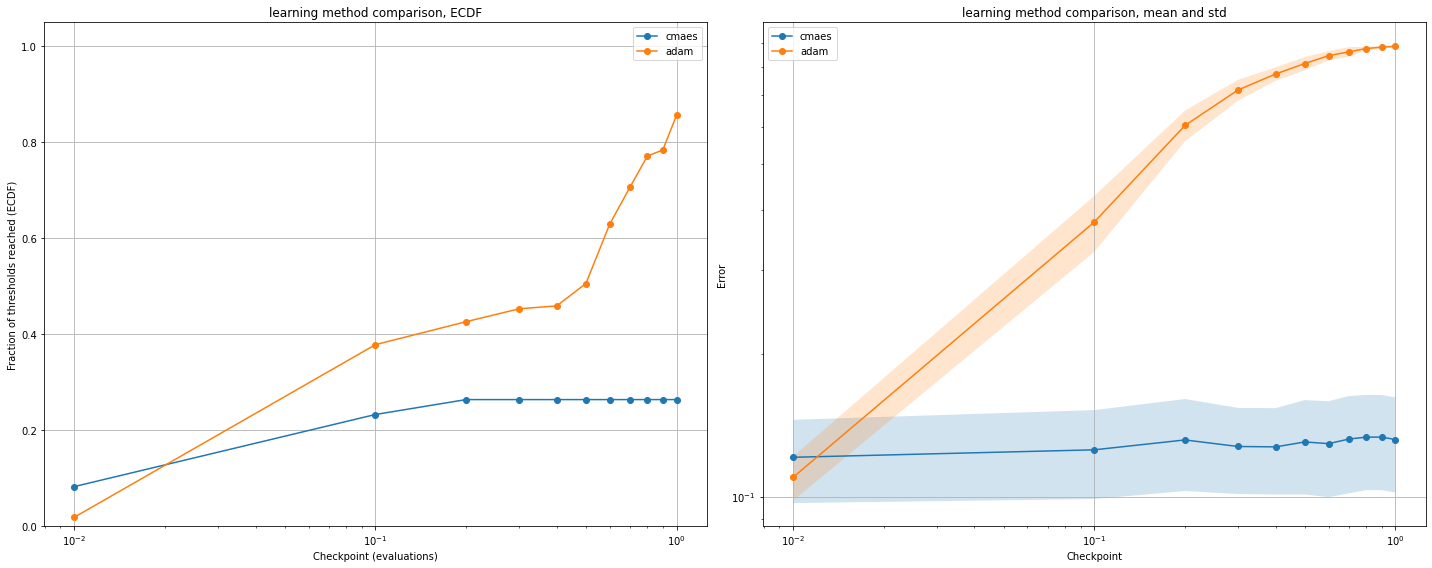
\includegraphics[height=4cm]{met_an//net//graphs/1.png}
\end{subfigure}
\caption{model przykładowej sieci neuronowej}

\label{fig:network_chart}
\end{figure}

\vspace{0.5em}

\begin{figure}[H]
\centering

\begin{subfigure}[c]{0.2\textwidth}
  \includegraphics[height=3cm]{met_an/cec/funkcje/F32013.png}
\end{subfigure}
\hfill
\begin{subfigure}[c]{0.7\textwidth}
  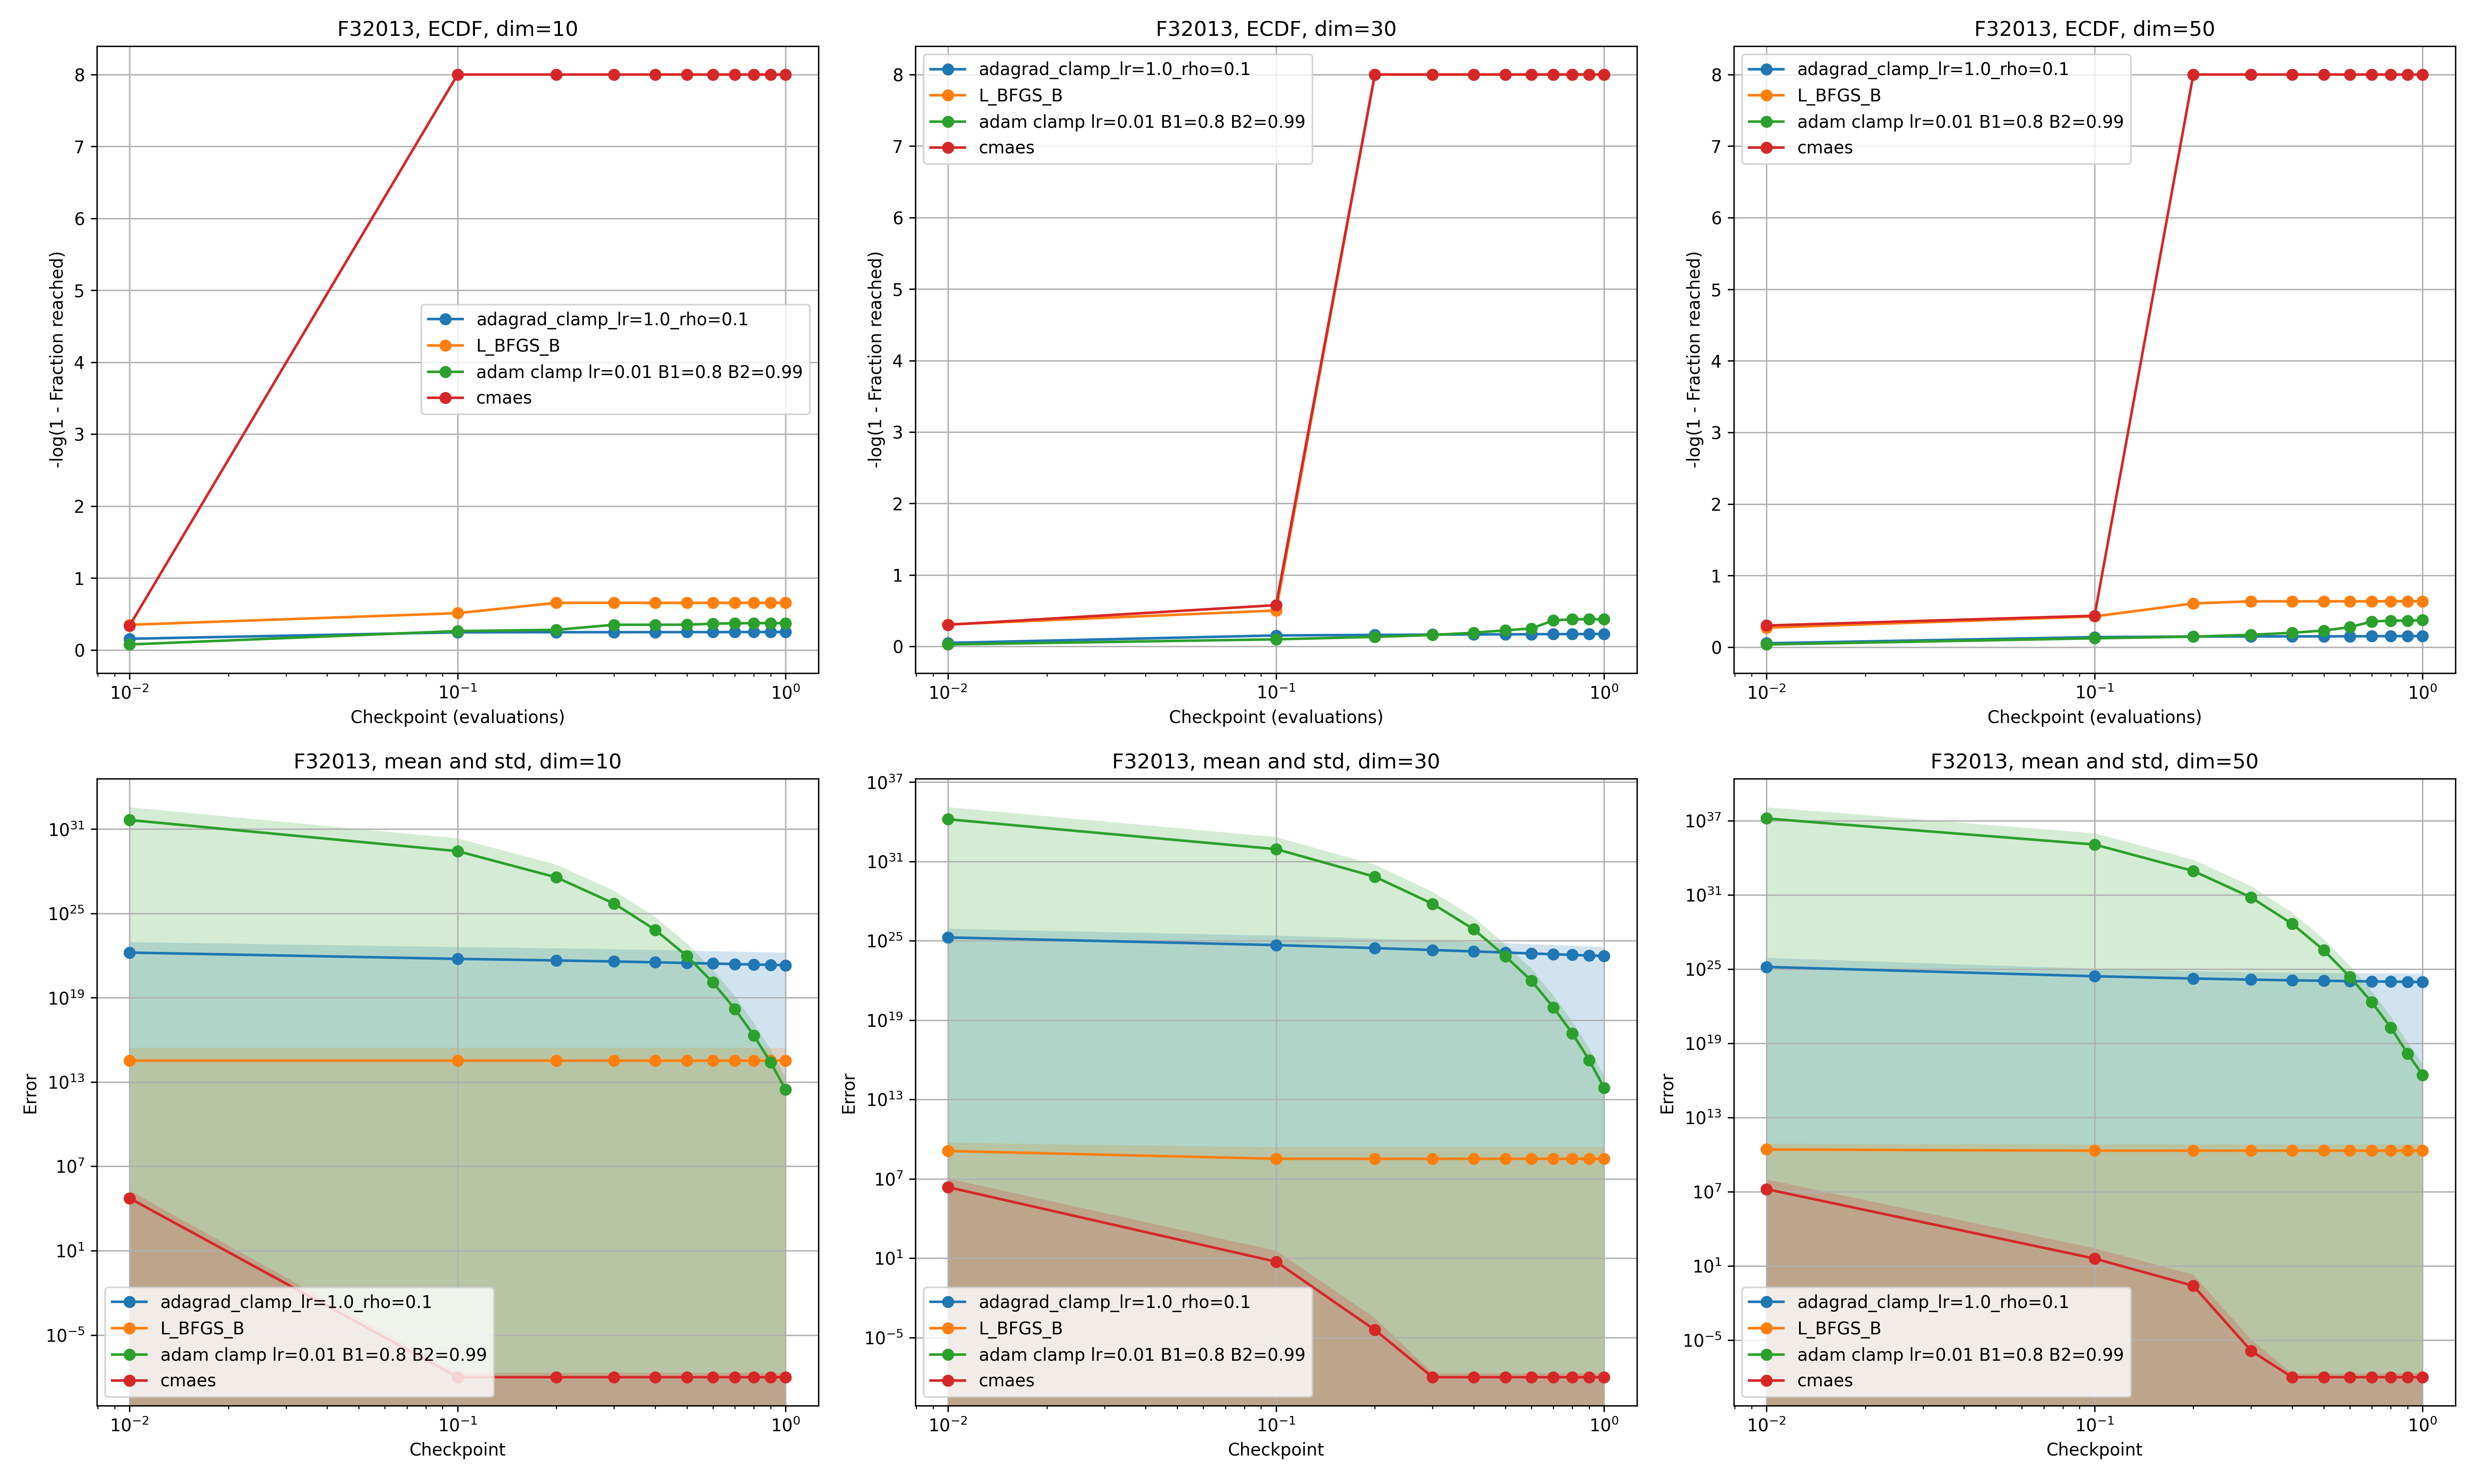
\includegraphics[height=6.5cm]{met_an/cec/funkcje/F32013_rec.png}
\end{subfigure}
\caption{F3 - Rotated Bent Cigar Function}

\vspace{0.5em}

\begin{subfigure}[c]{0.2\textwidth}
  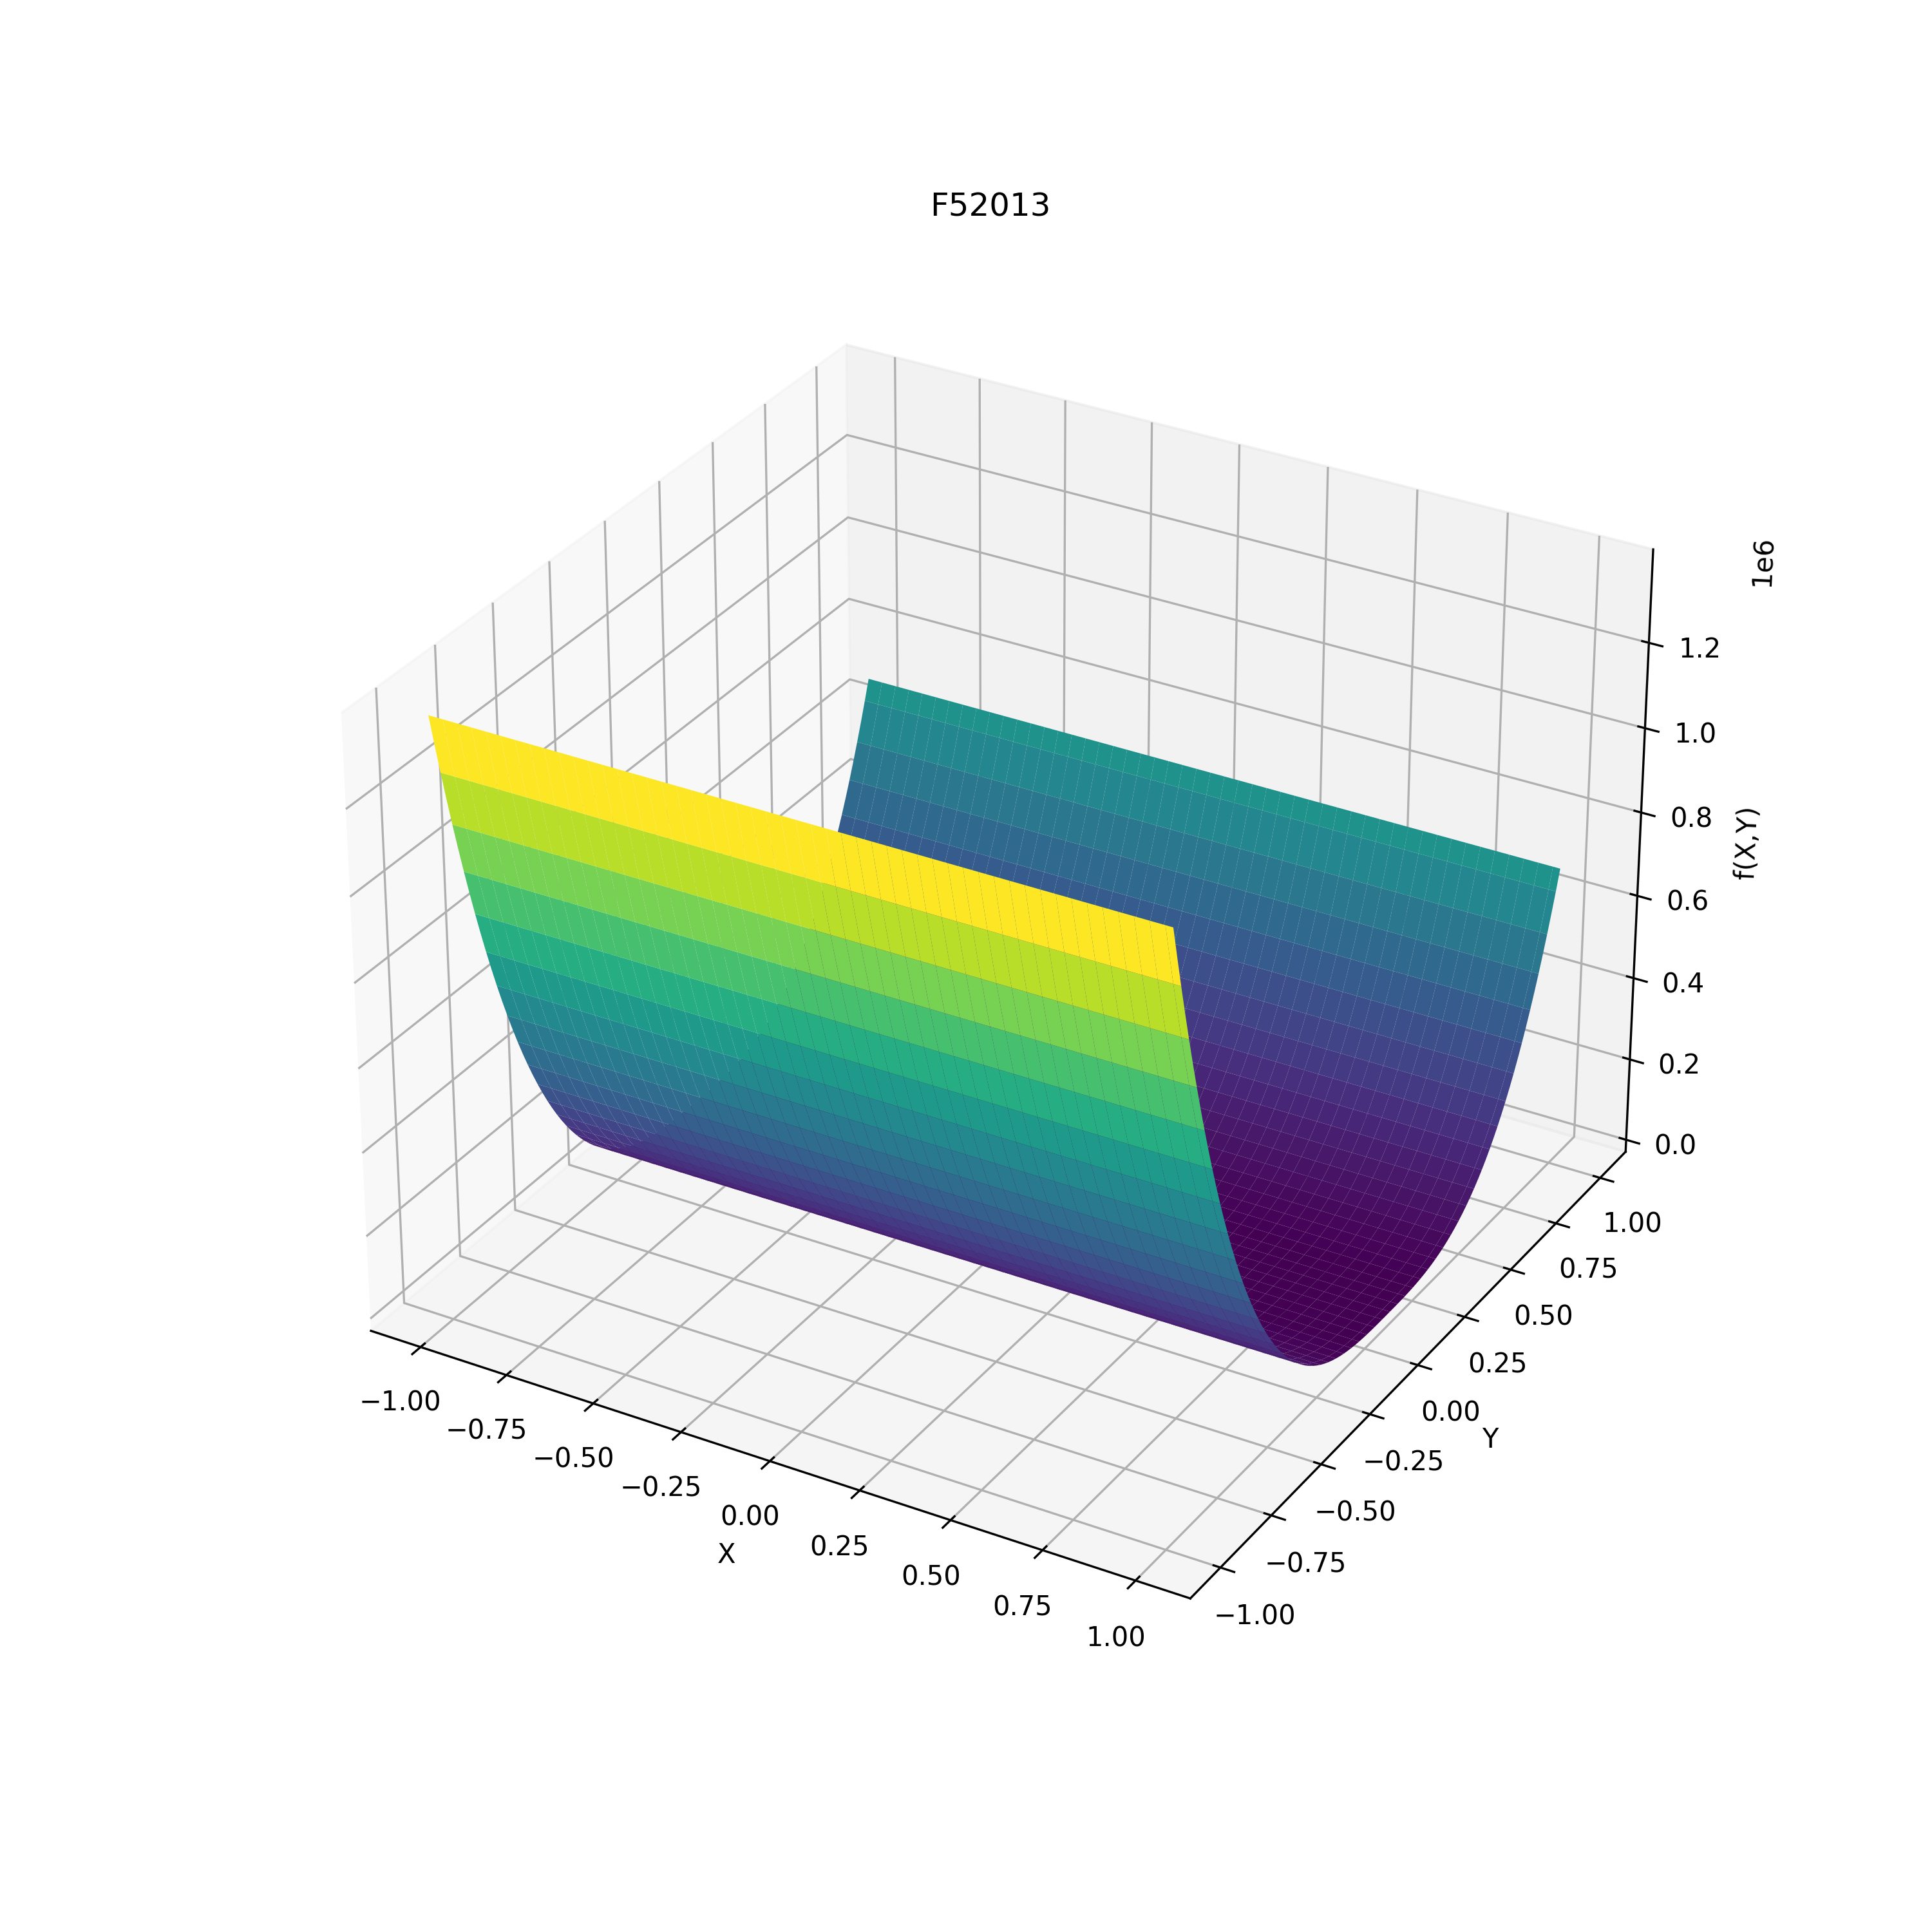
\includegraphics[height=3cm]{met_an/cec/funkcje/F52013.png}
\end{subfigure}
\hfill
\begin{subfigure}[c]{0.7\textwidth}
  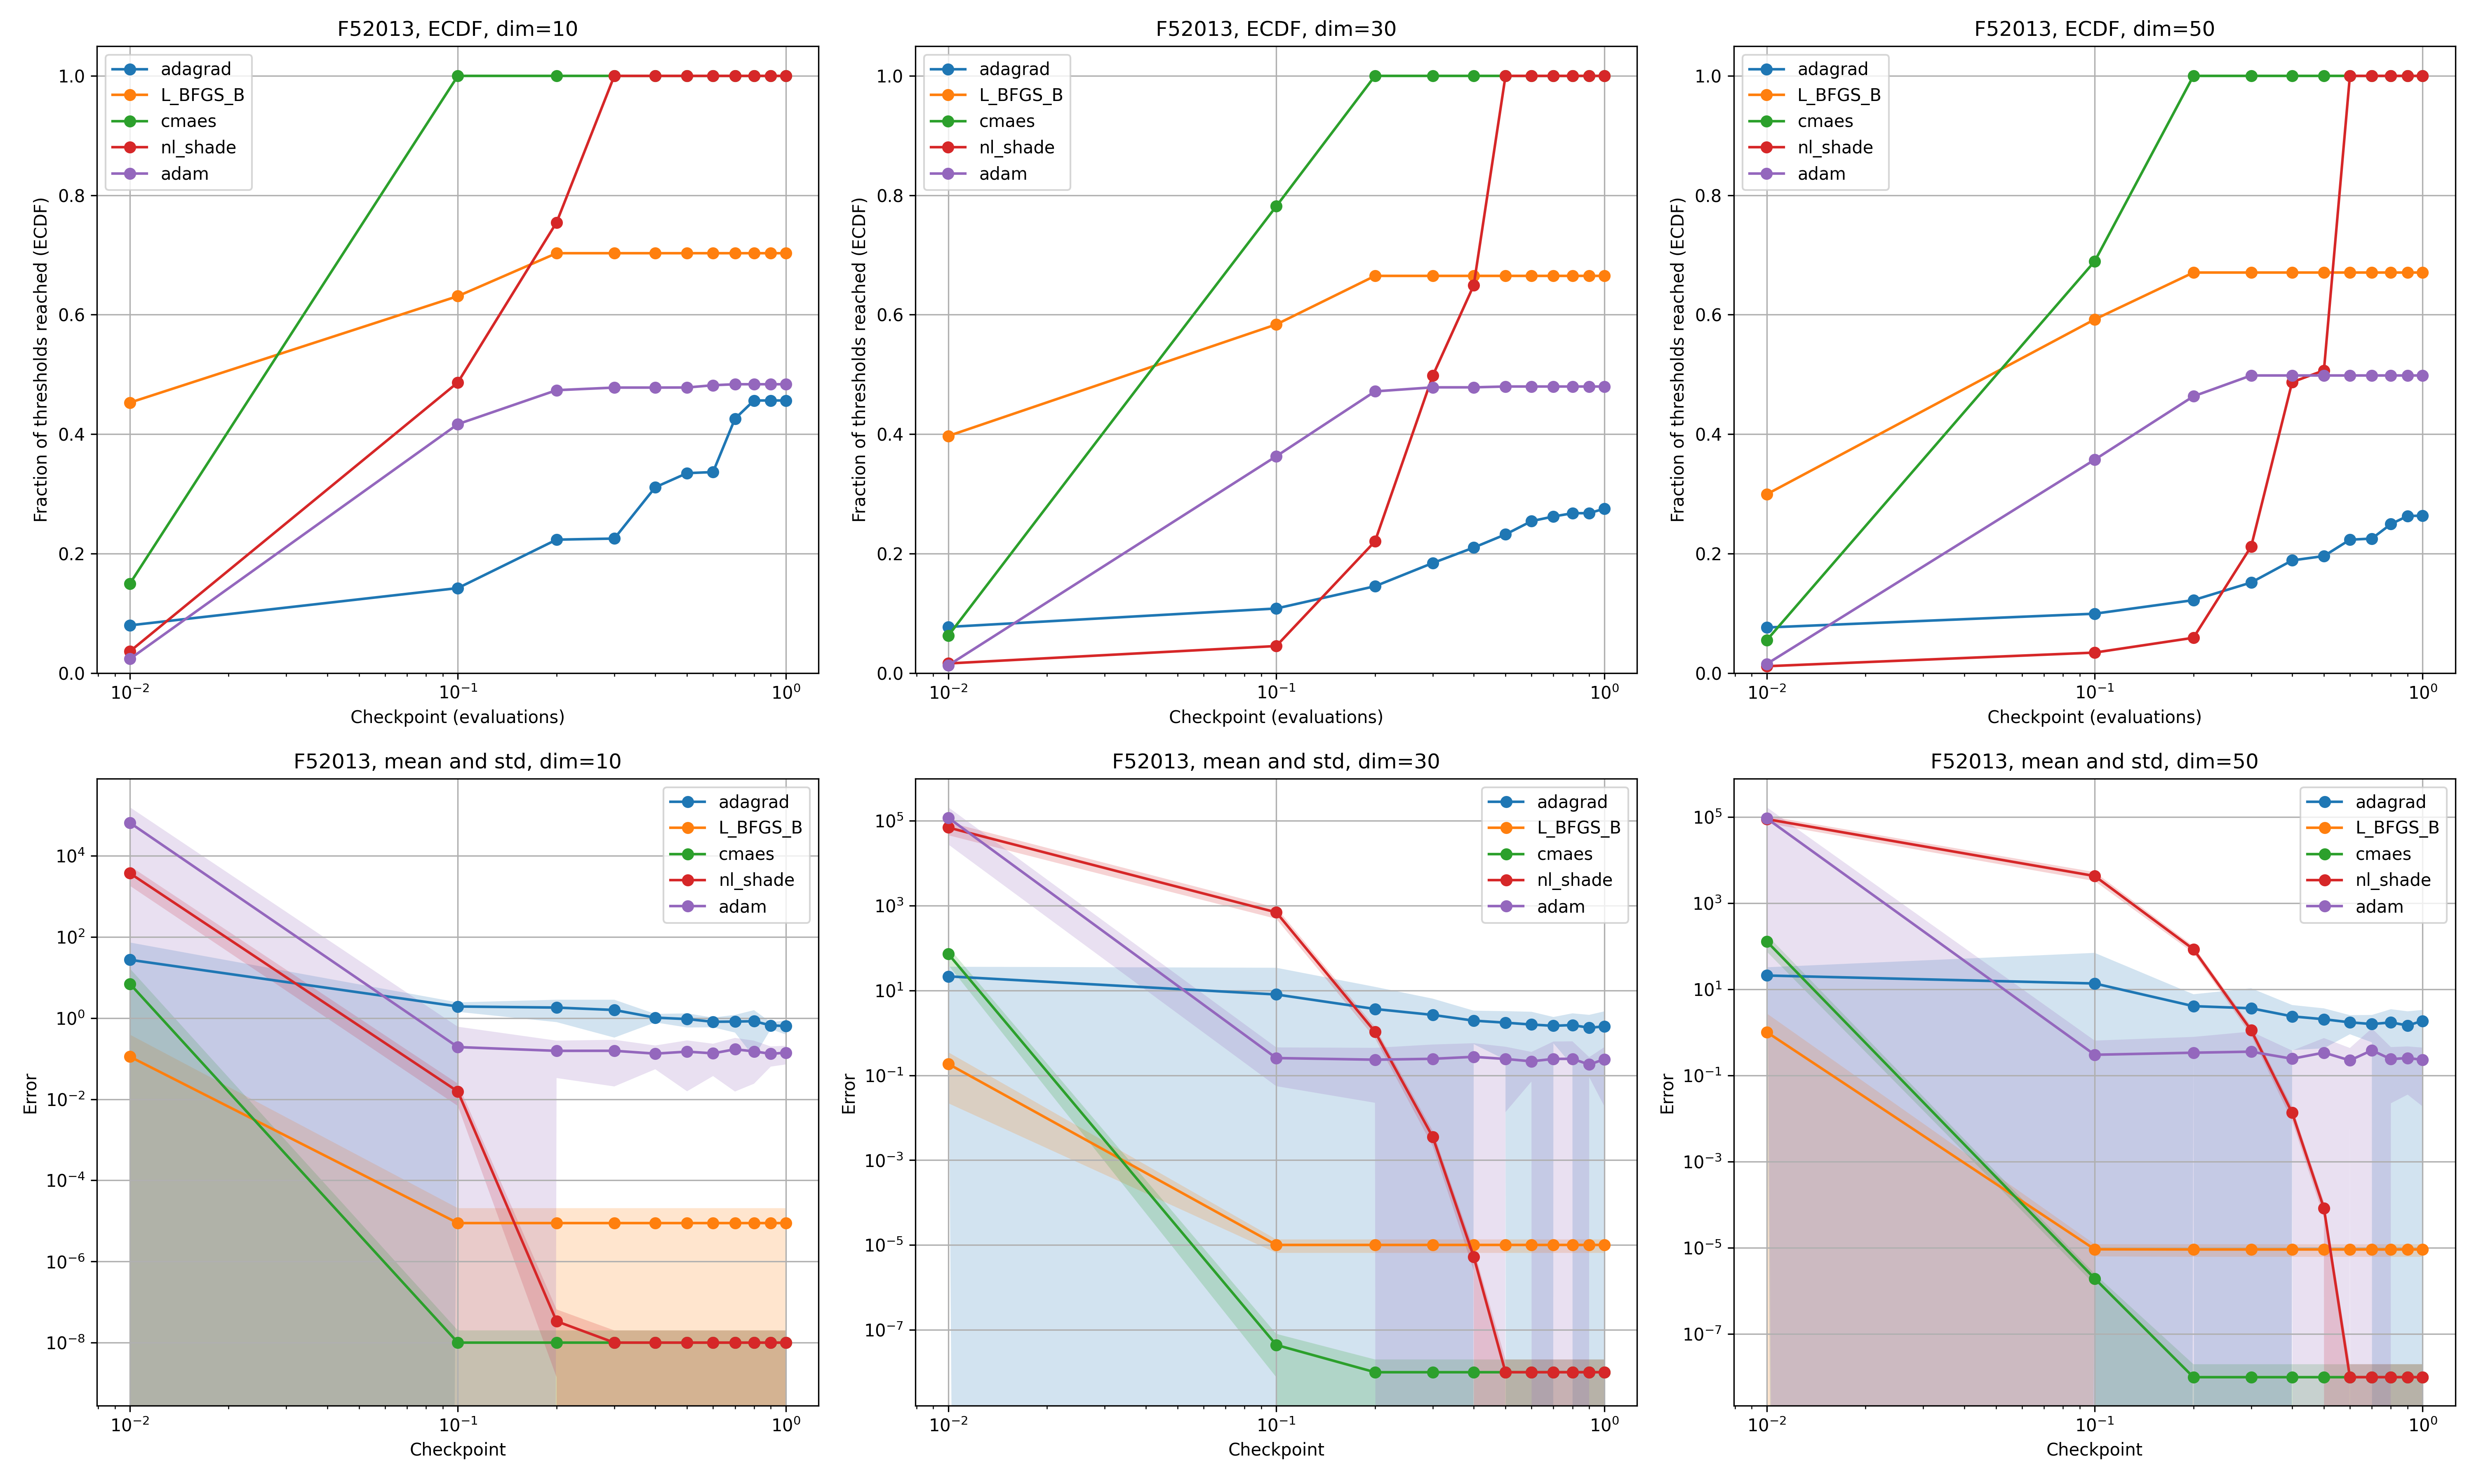
\includegraphics[height=6.5cm]{met_an/cec/funkcje/F52013_rec.png}
\end{subfigure}
\caption{F5 - Different Powers Function}

\vspace{0.5em}

\begin{subfigure}[c]{0.2\textwidth}
  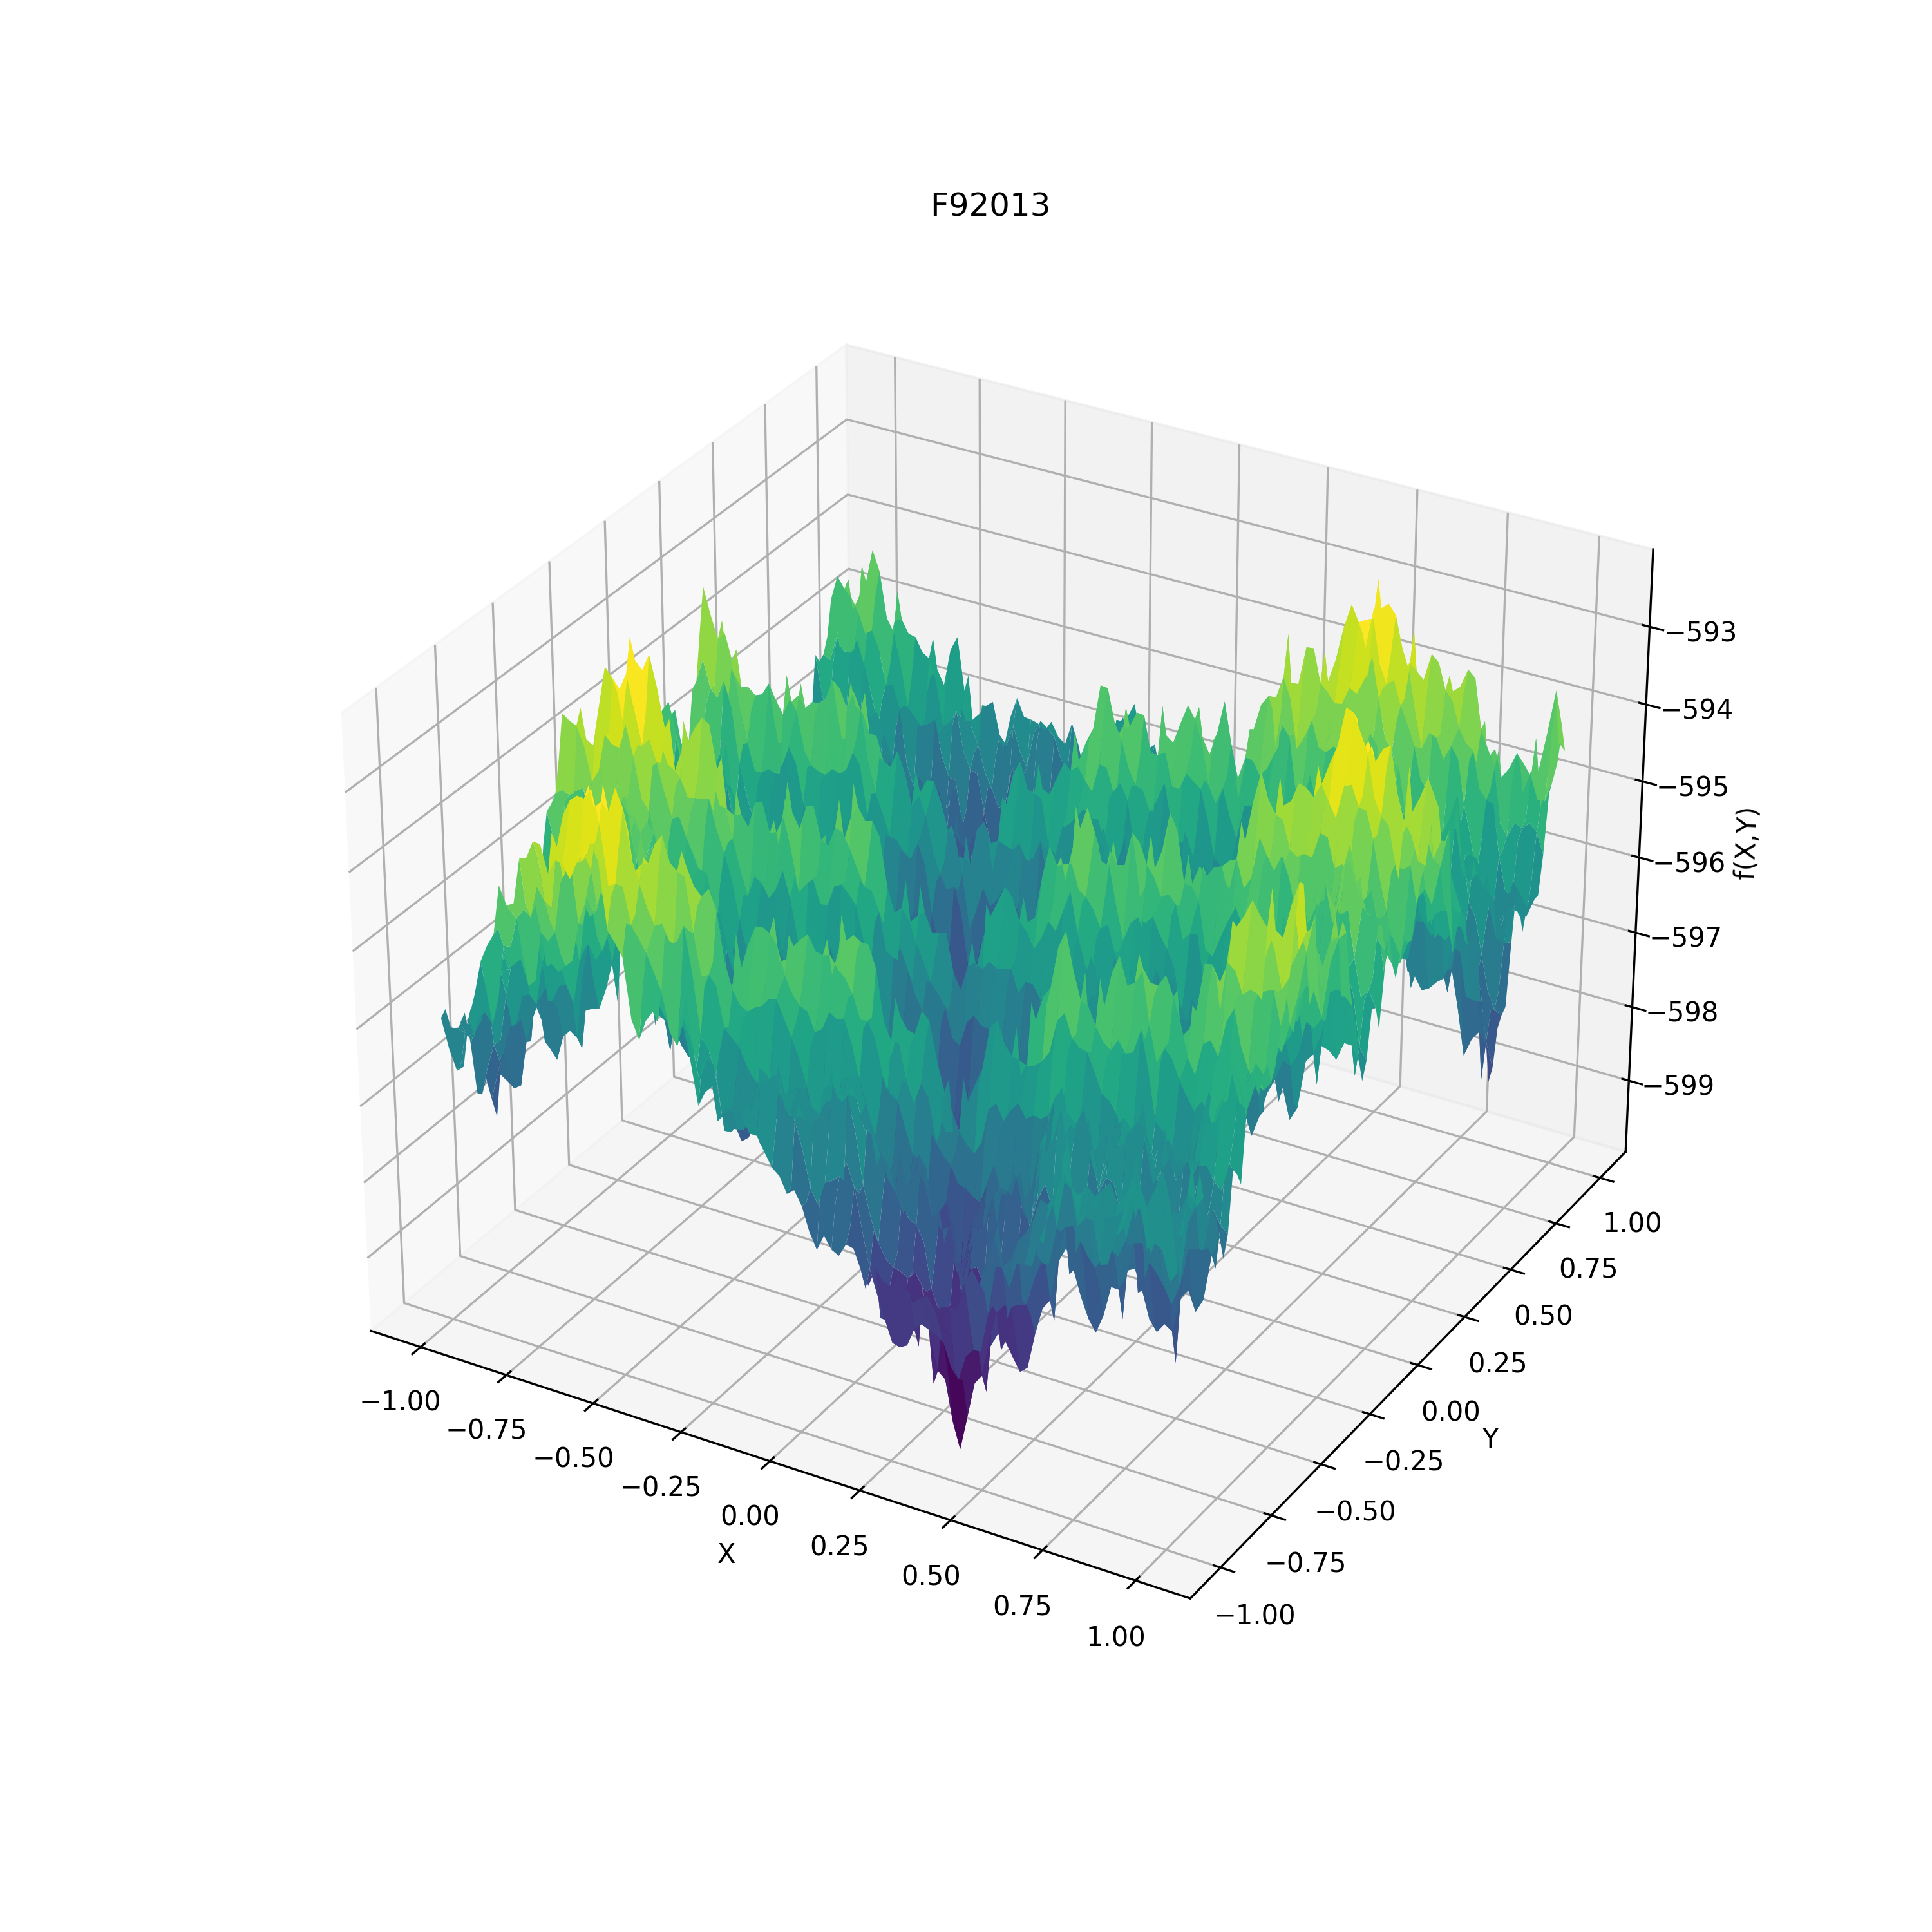
\includegraphics[height=3cm]{met_an/cec/funkcje/F92013.png}
\end{subfigure}
\hfill
\begin{subfigure}[c]{0.7\textwidth}
  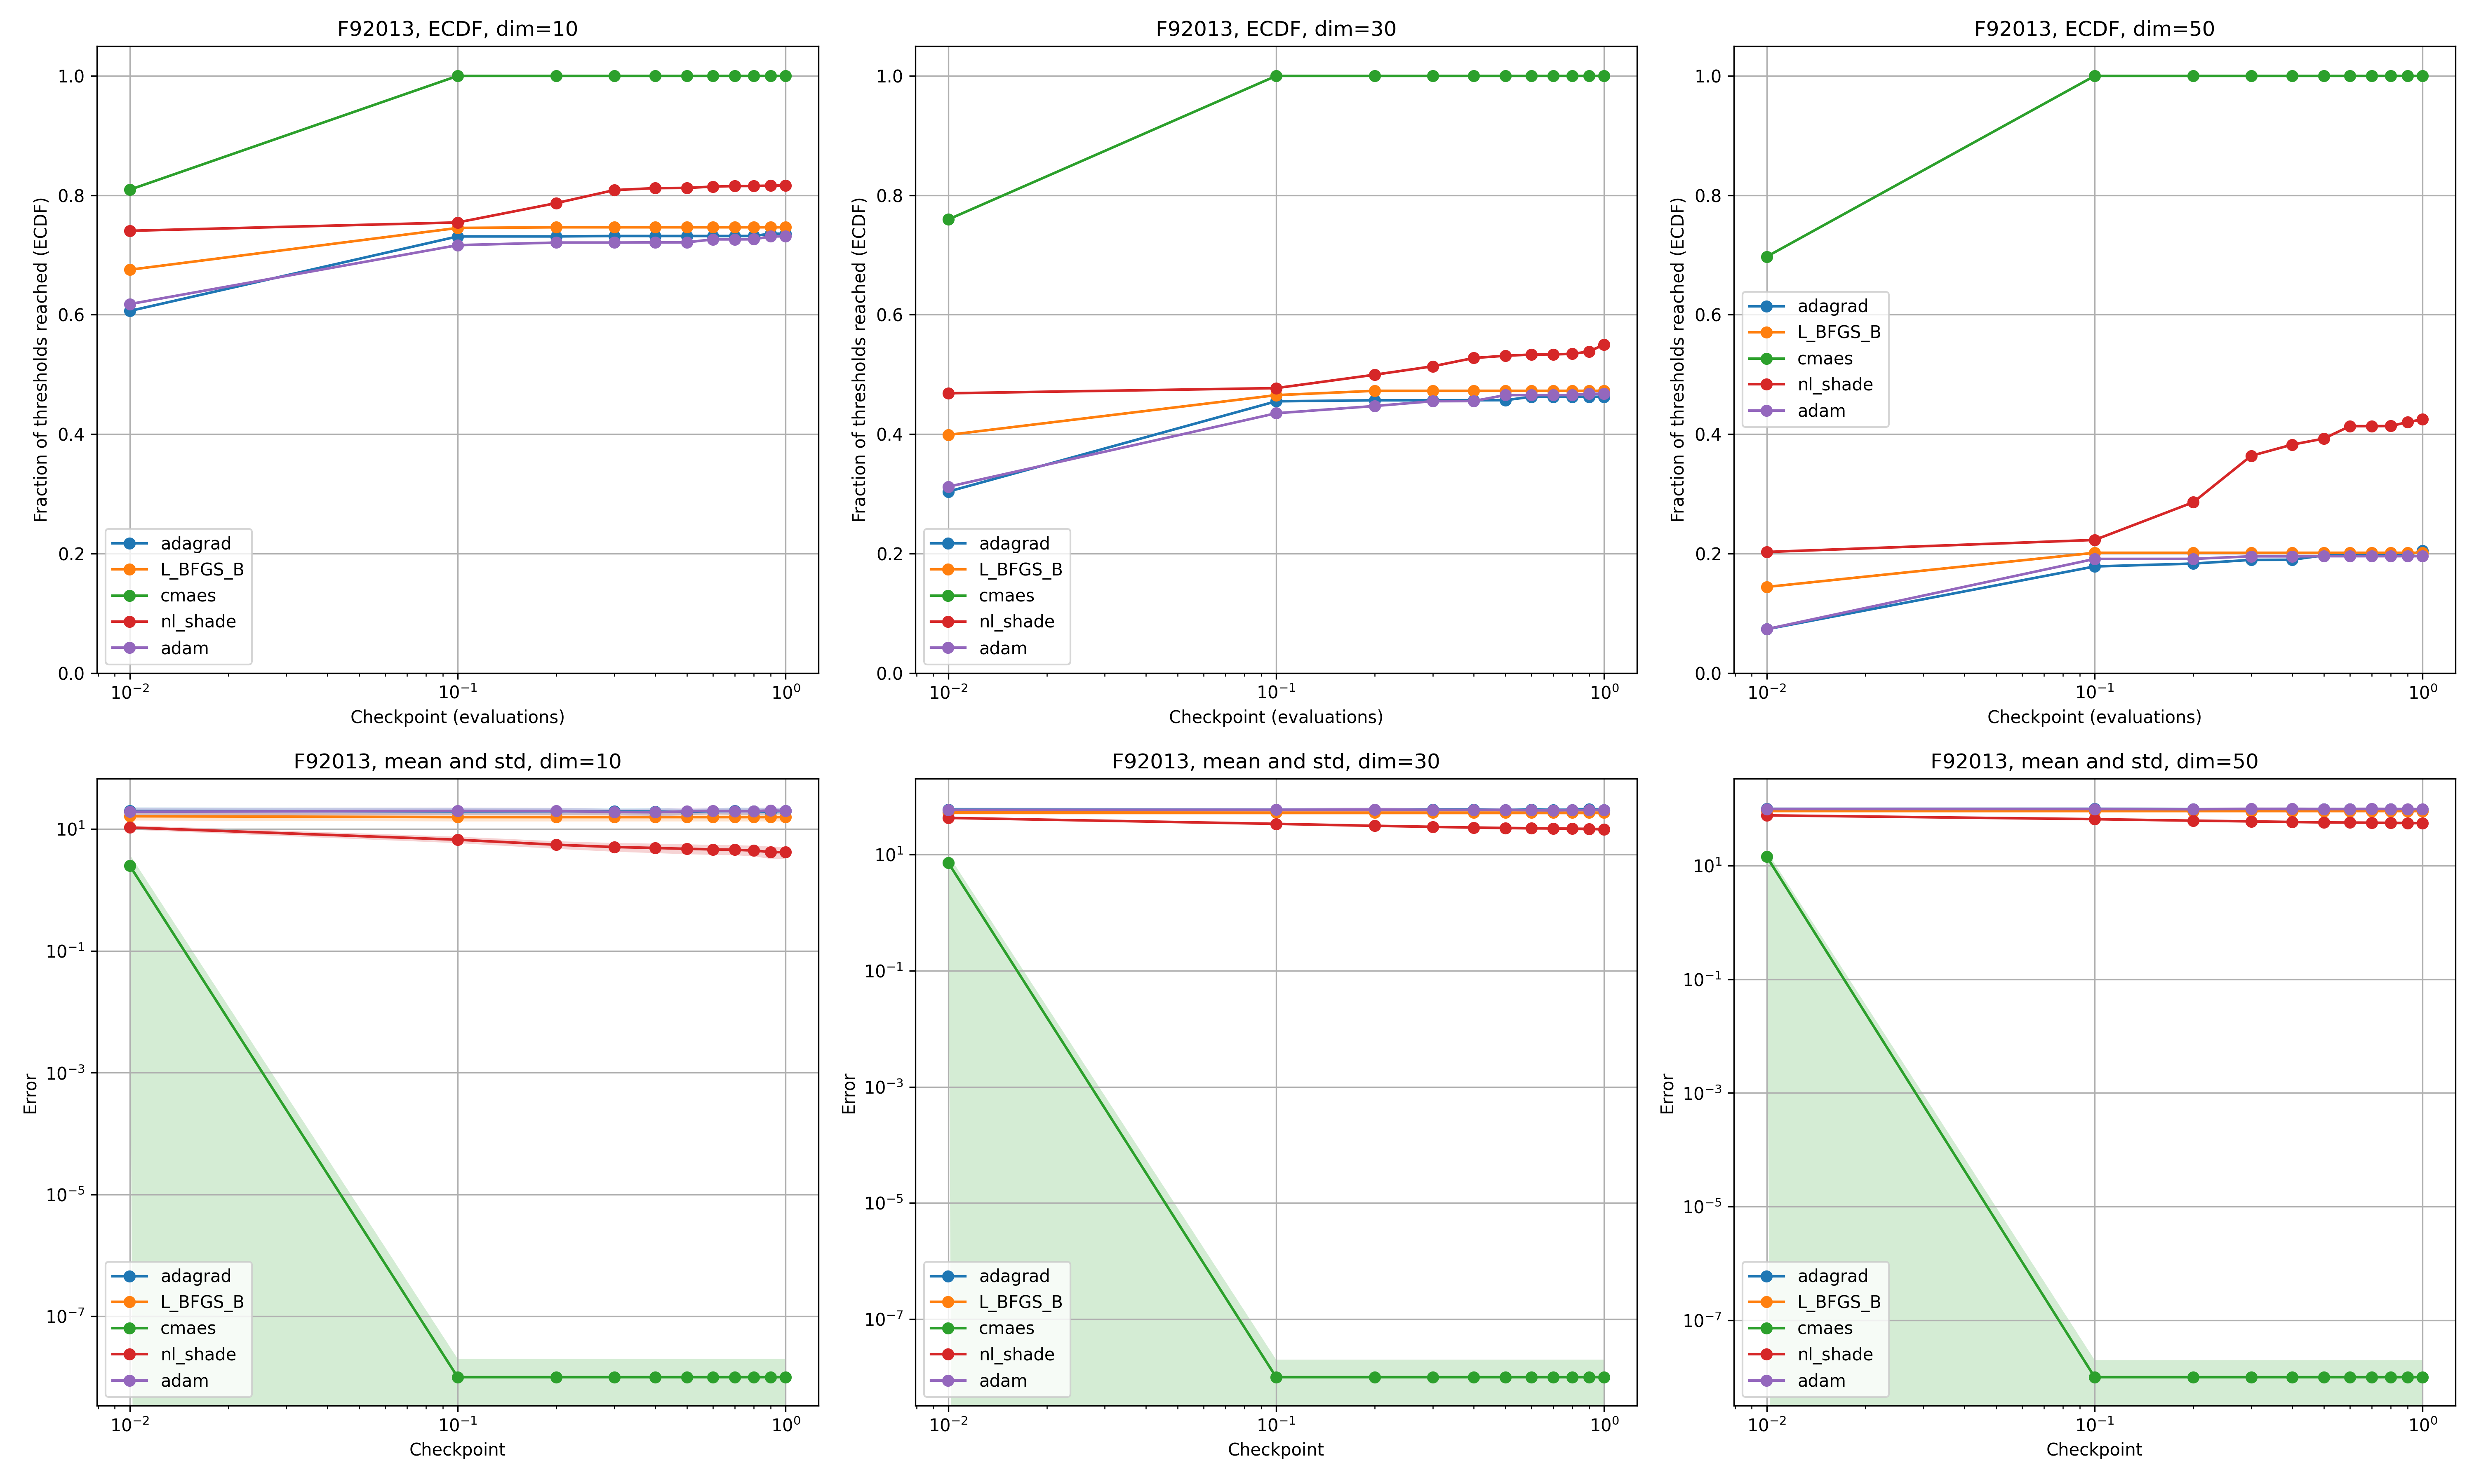
\includegraphics[height=6.5cm]{met_an/cec/funkcje/F92013_rec.png}
\end{subfigure}
\caption{F9 - Rotated Weierstrass Function}

\vspace{0.5em}

\label{fig:allfunc}
\end{figure}

\begin{figure}[H]
\centering

\begin{subfigure}[c]{0.2\textwidth}
  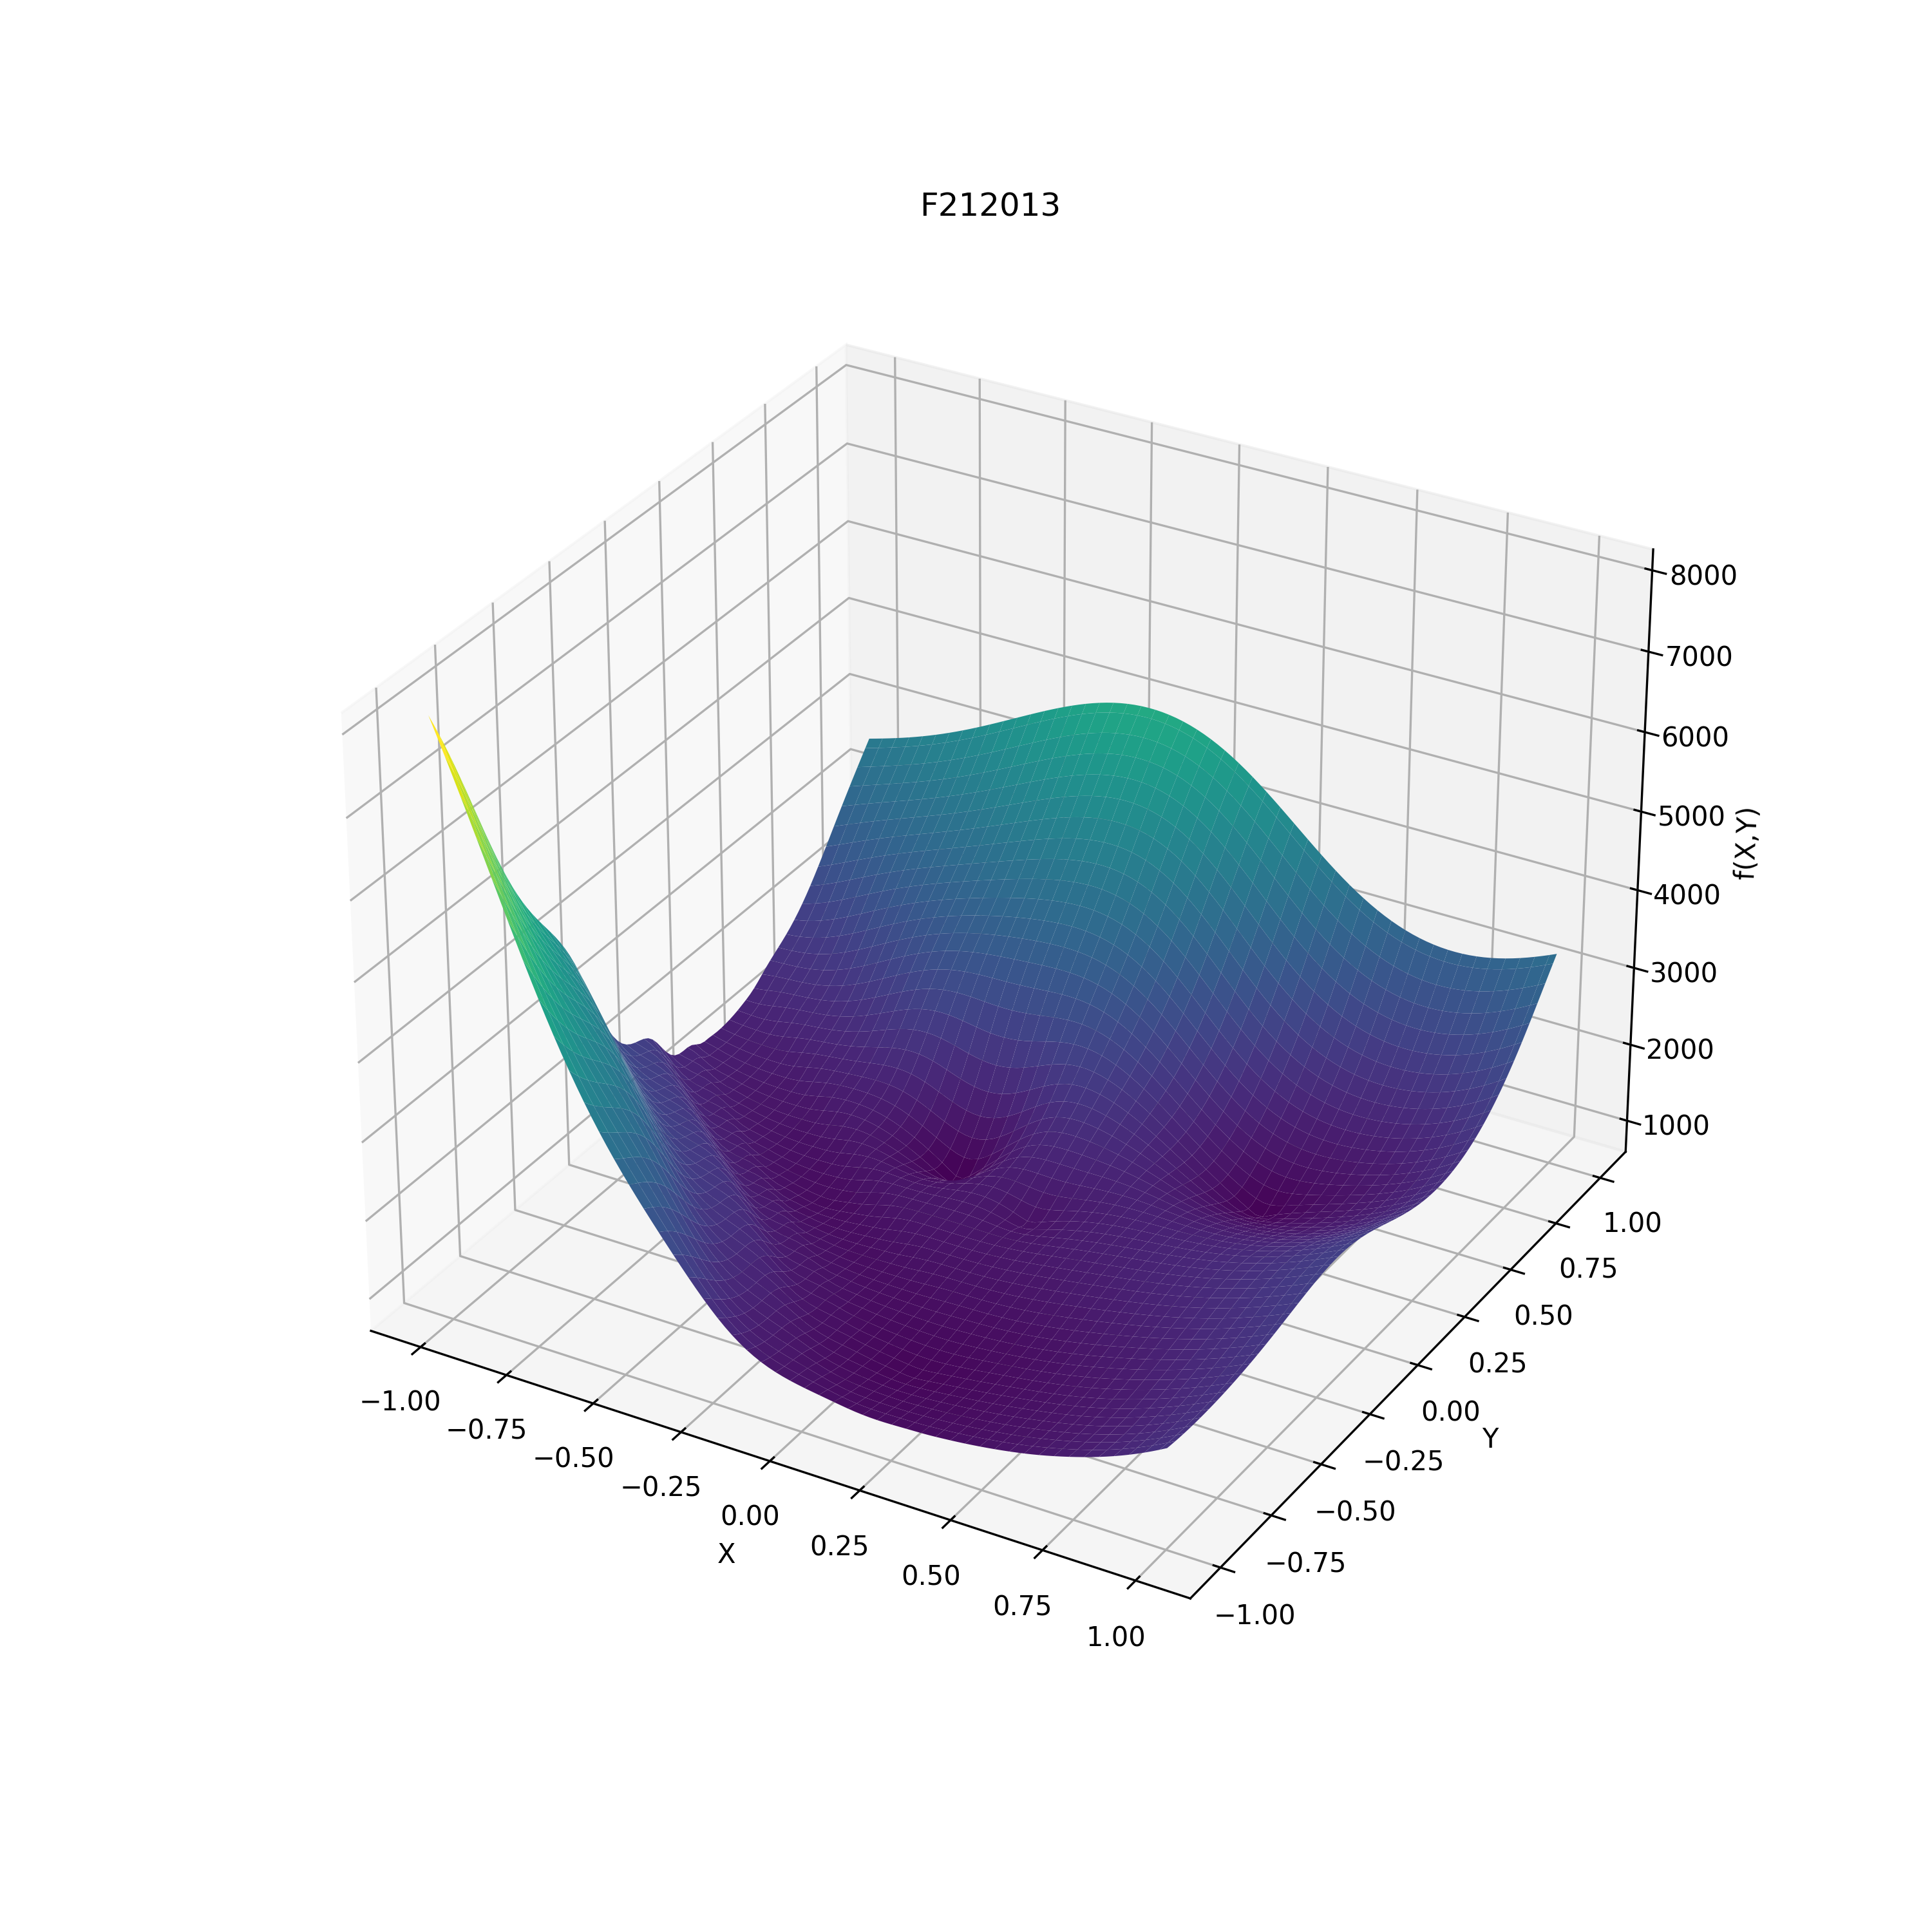
\includegraphics[height=3cm]{met_an/cec/funkcje/F212013.png}
\end{subfigure}
\hfill
\begin{subfigure}[c]{0.7\textwidth}
  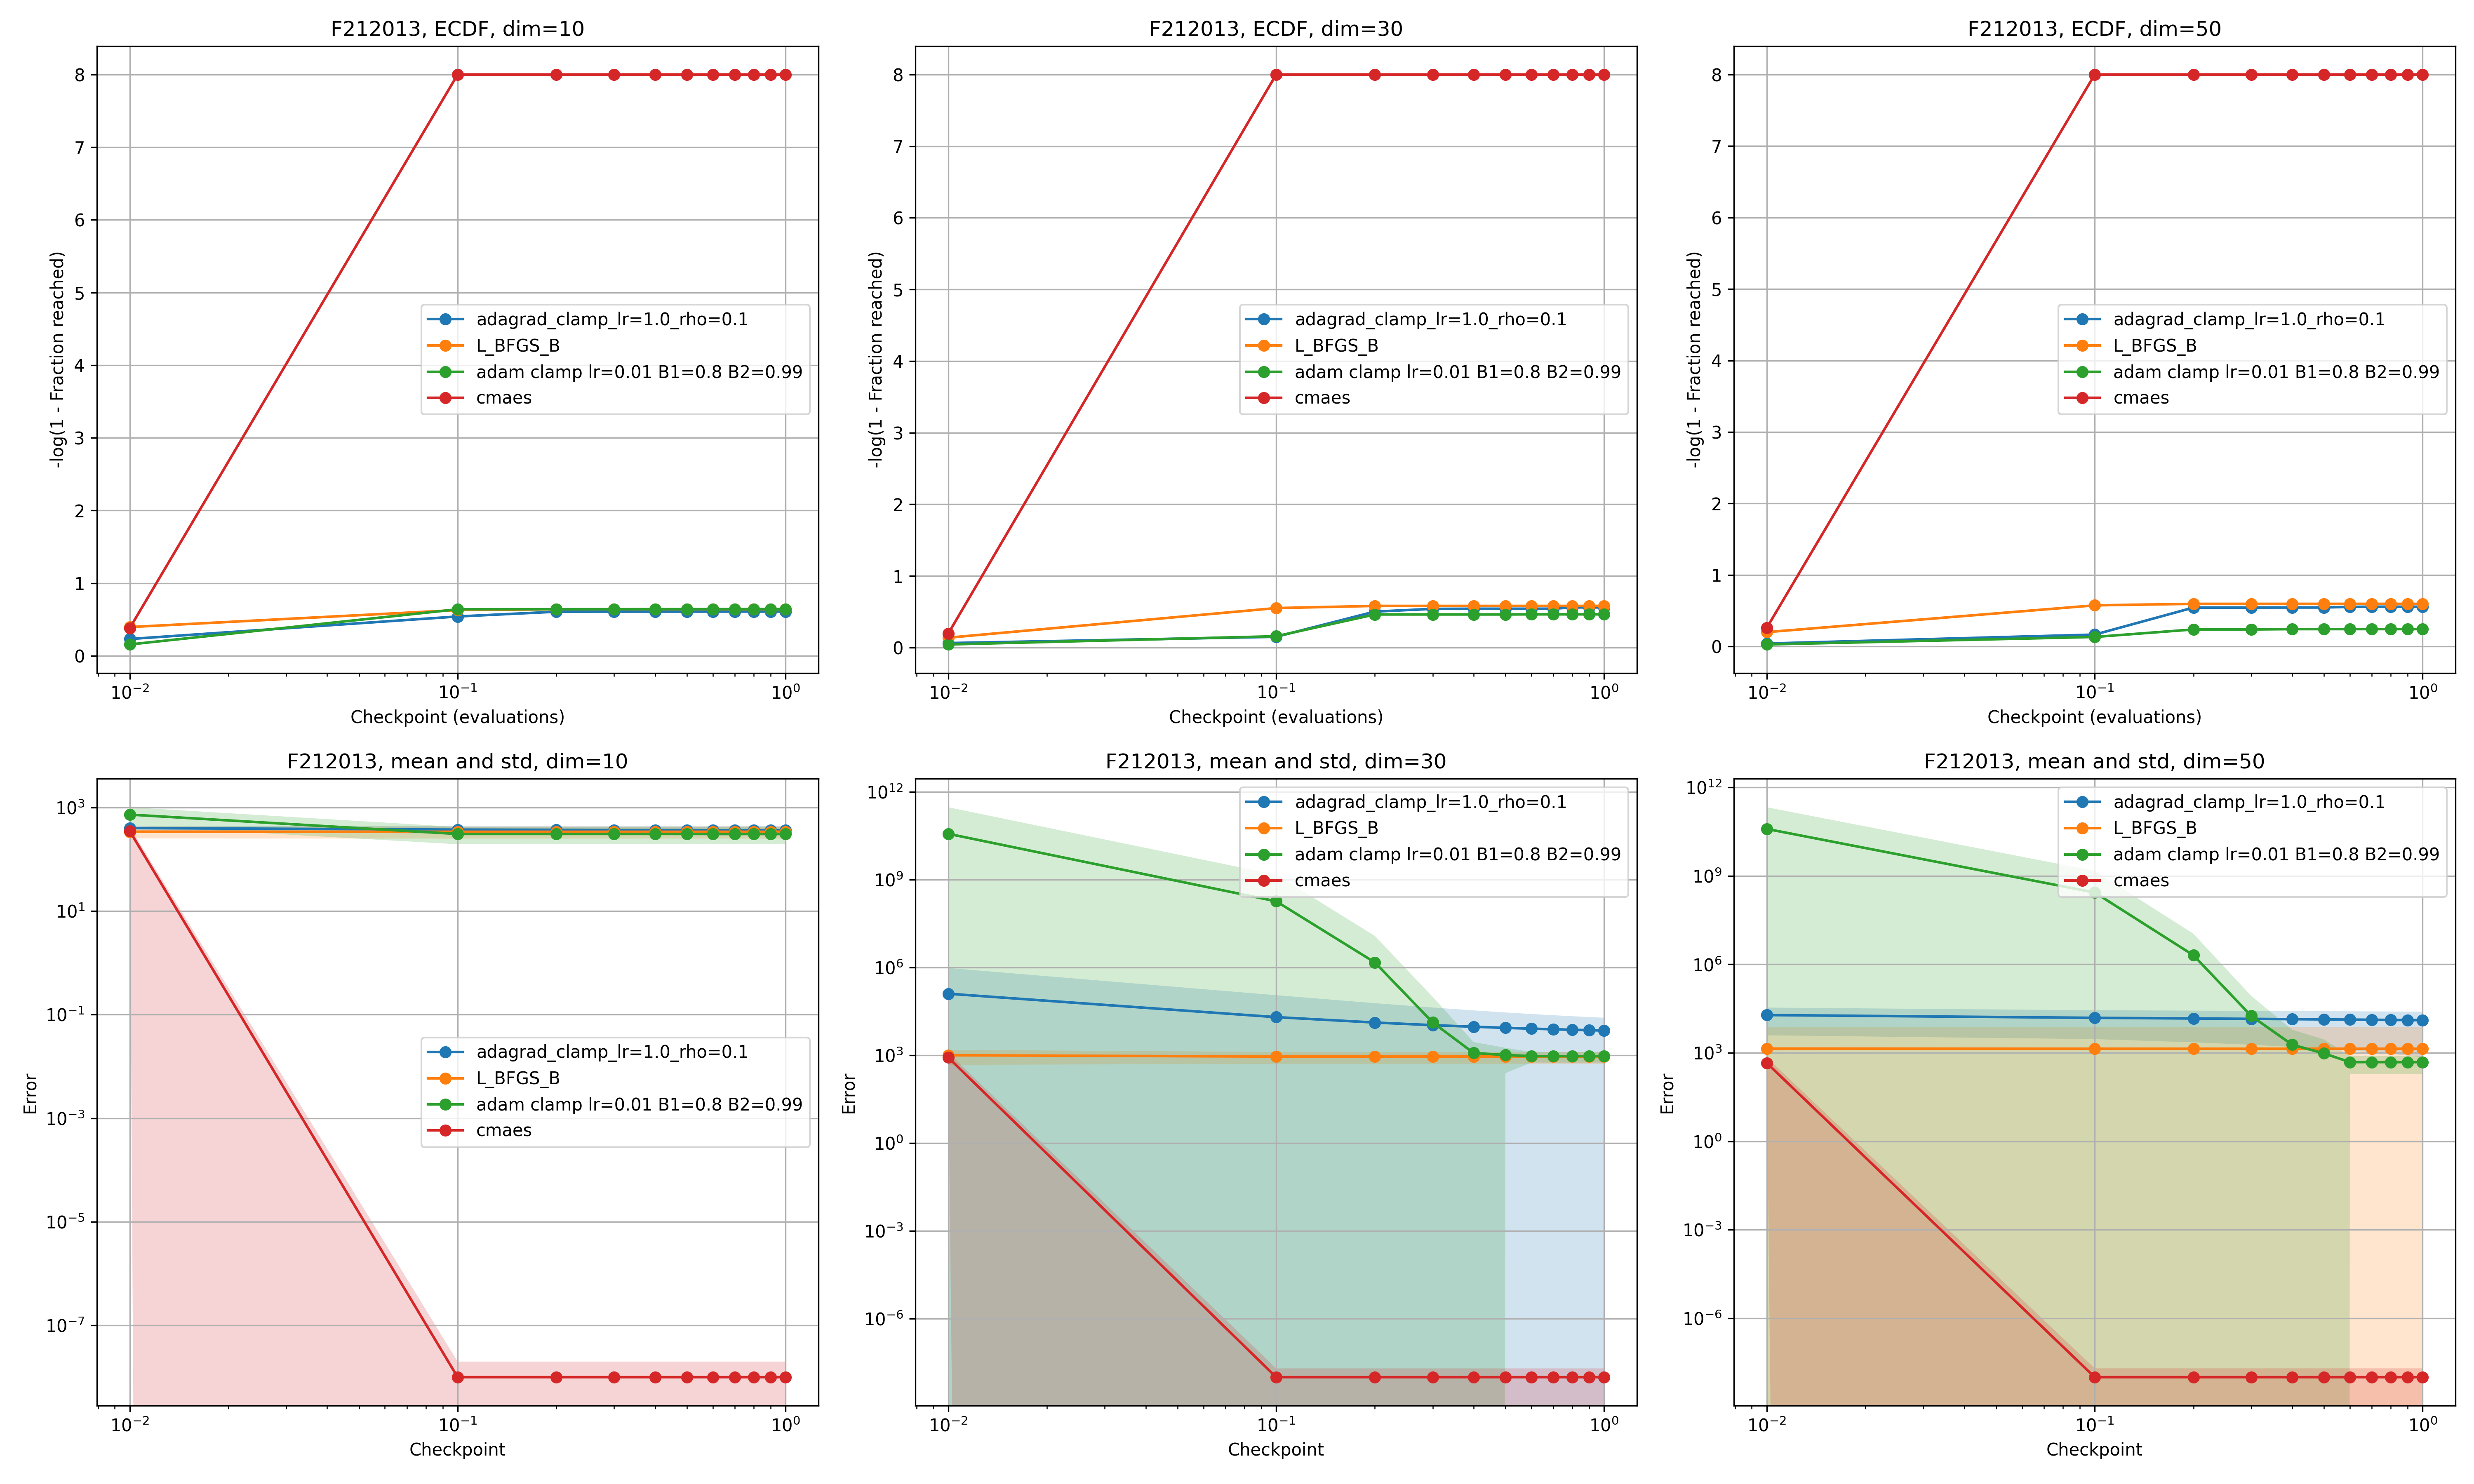
\includegraphics[height=6.5cm]{met_an/cec/funkcje/F212013_rec.png}
\end{subfigure}
\caption{F21 - Composition Function 1 (n=5,Rotated)}

\label{fig:allfunc_page_2}
\end{figure}












% \begin{figure}[H]
%     \centering
%     \begin{subfigure}[c]{0.2\textwidth}
%         \centering
%         \includegraphics[height=3cm, keepaspectratio]{met_an//cec//funkcje/F32013.png}
%     \end{subfigure}
%     \hfill
%     \begin{subfigure}[c]{0.7\textwidth}
%         \centering
%         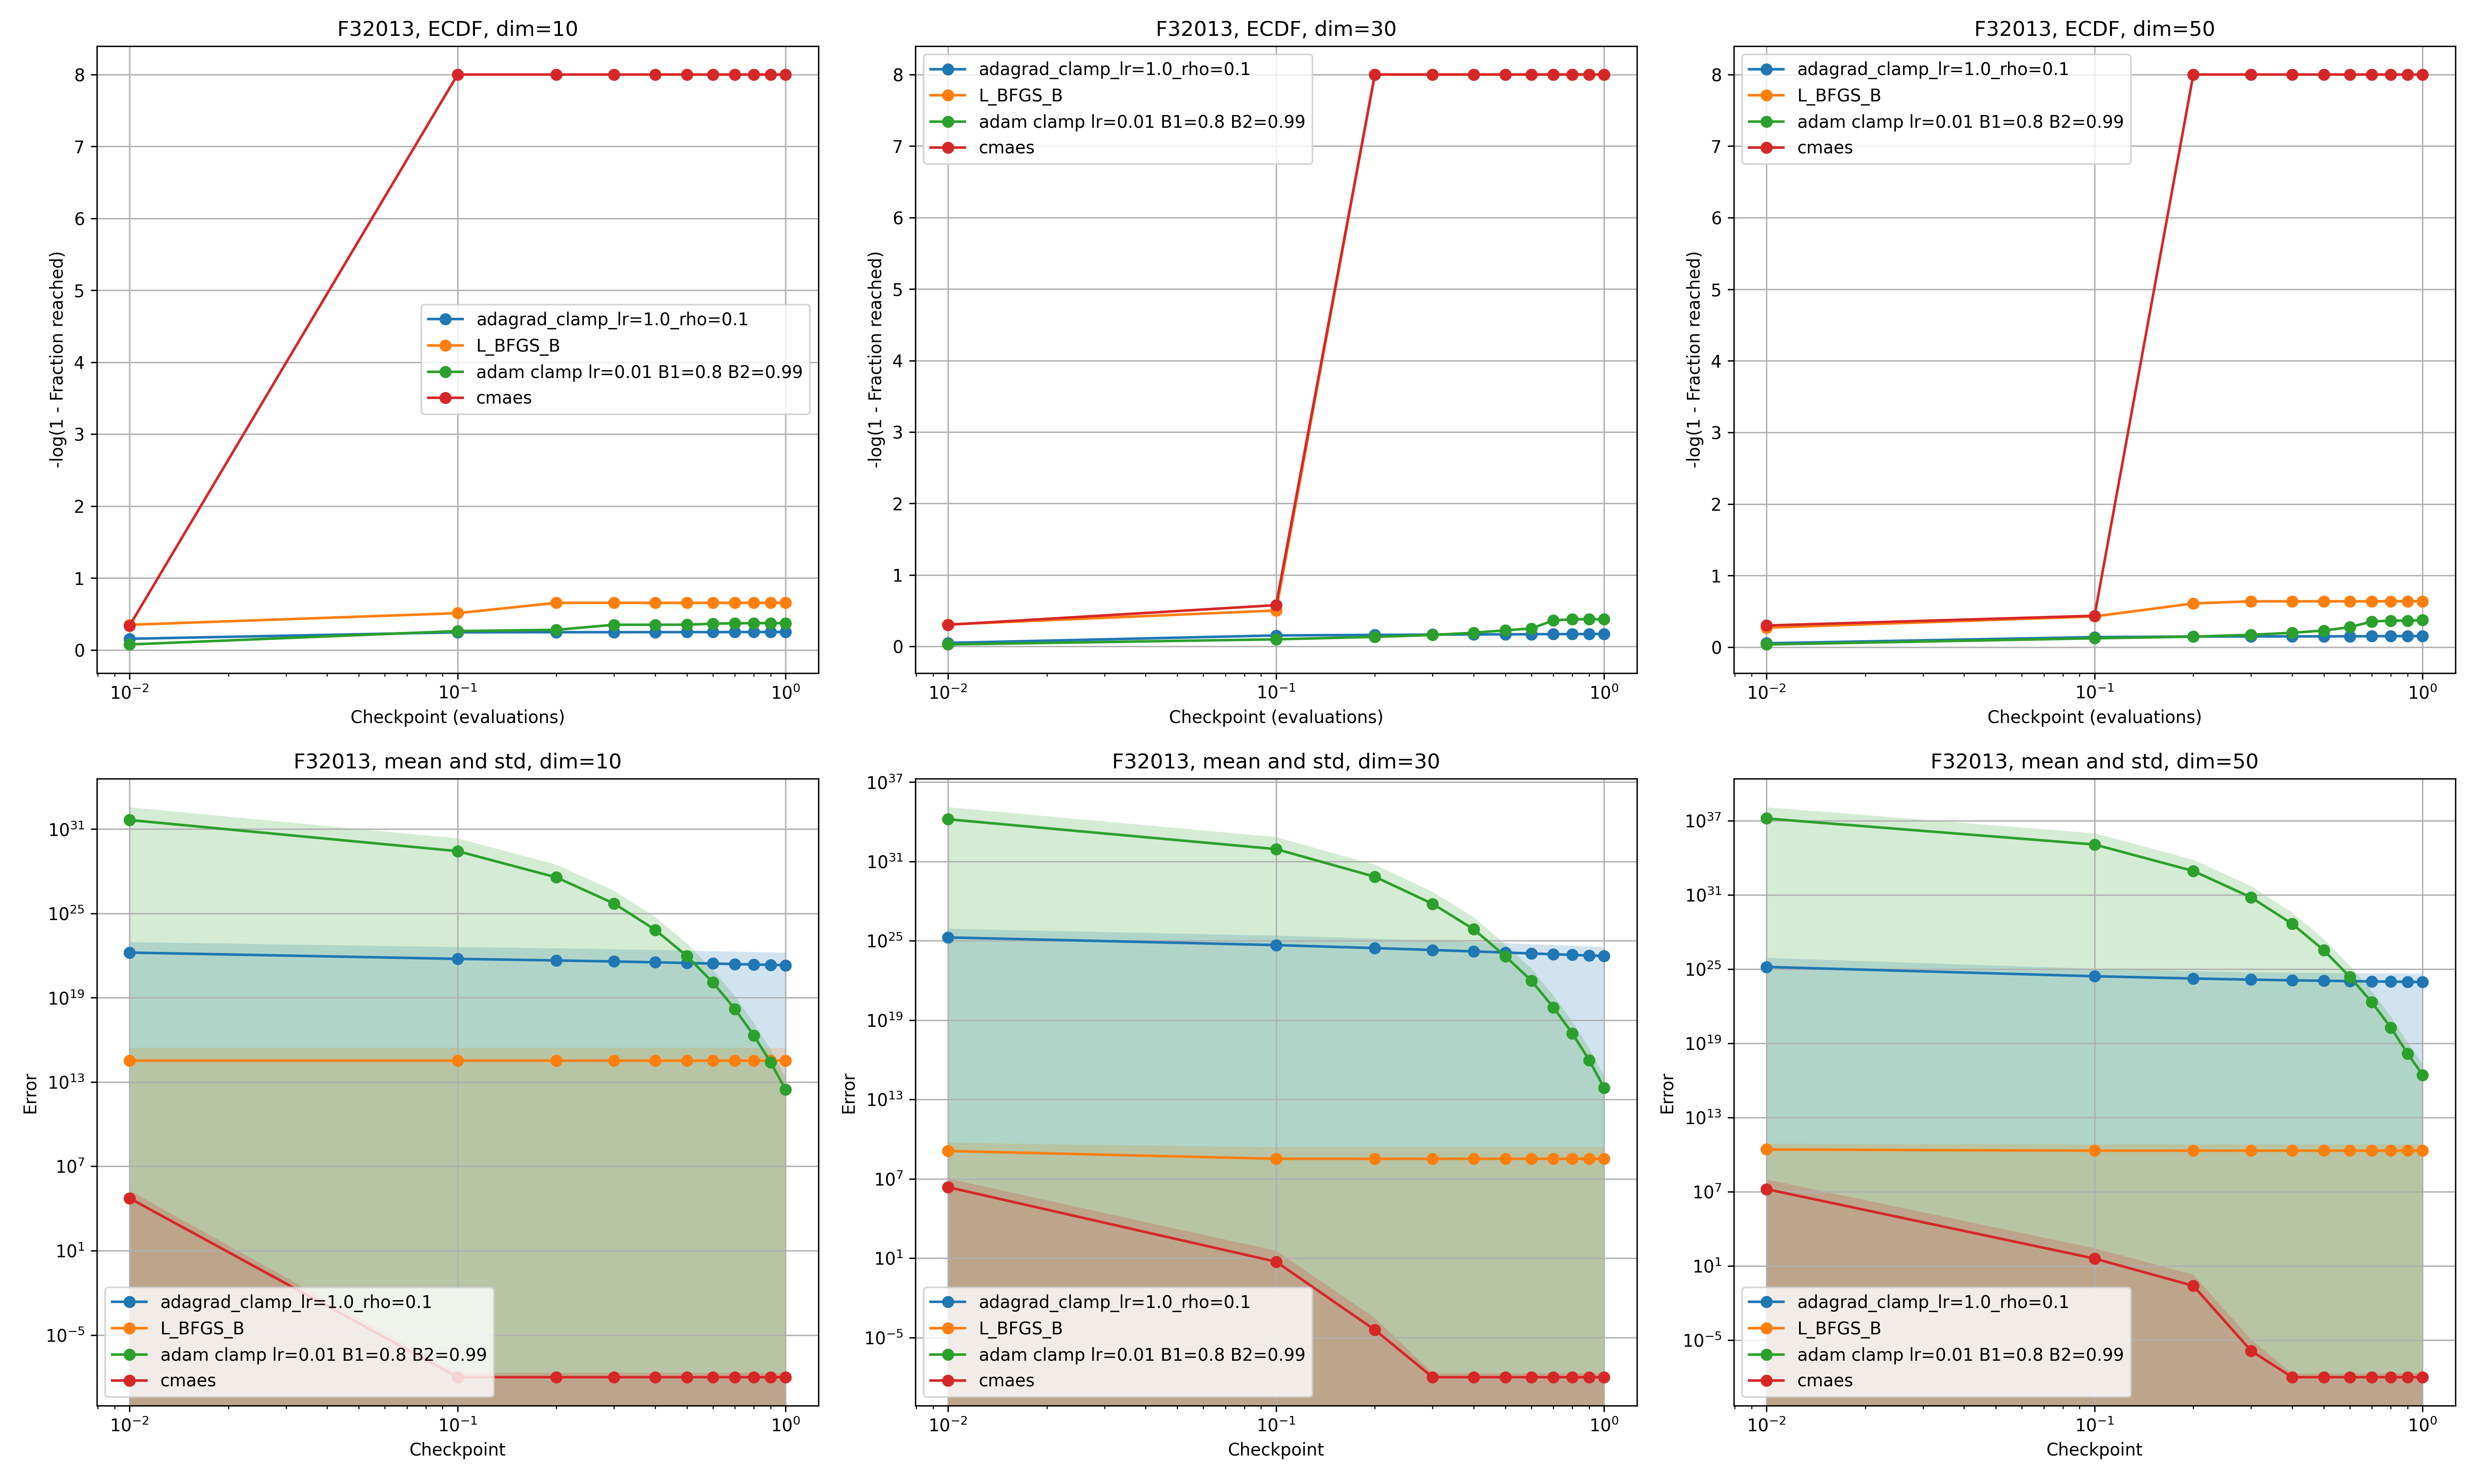
\includegraphics[height=6.5cm, keepaspectratio]{met_an/cec/funkcje/F32013_rec.png}
%     \end{subfigure}
%     \caption{Rotated Bent Cigar Function}
%     \label{fig:F32013}
% \end{figure}

% \begin{figure}[H]
%     \centering
%     \begin{subfigure}[c]{0.2\textwidth}
%         \centering
%         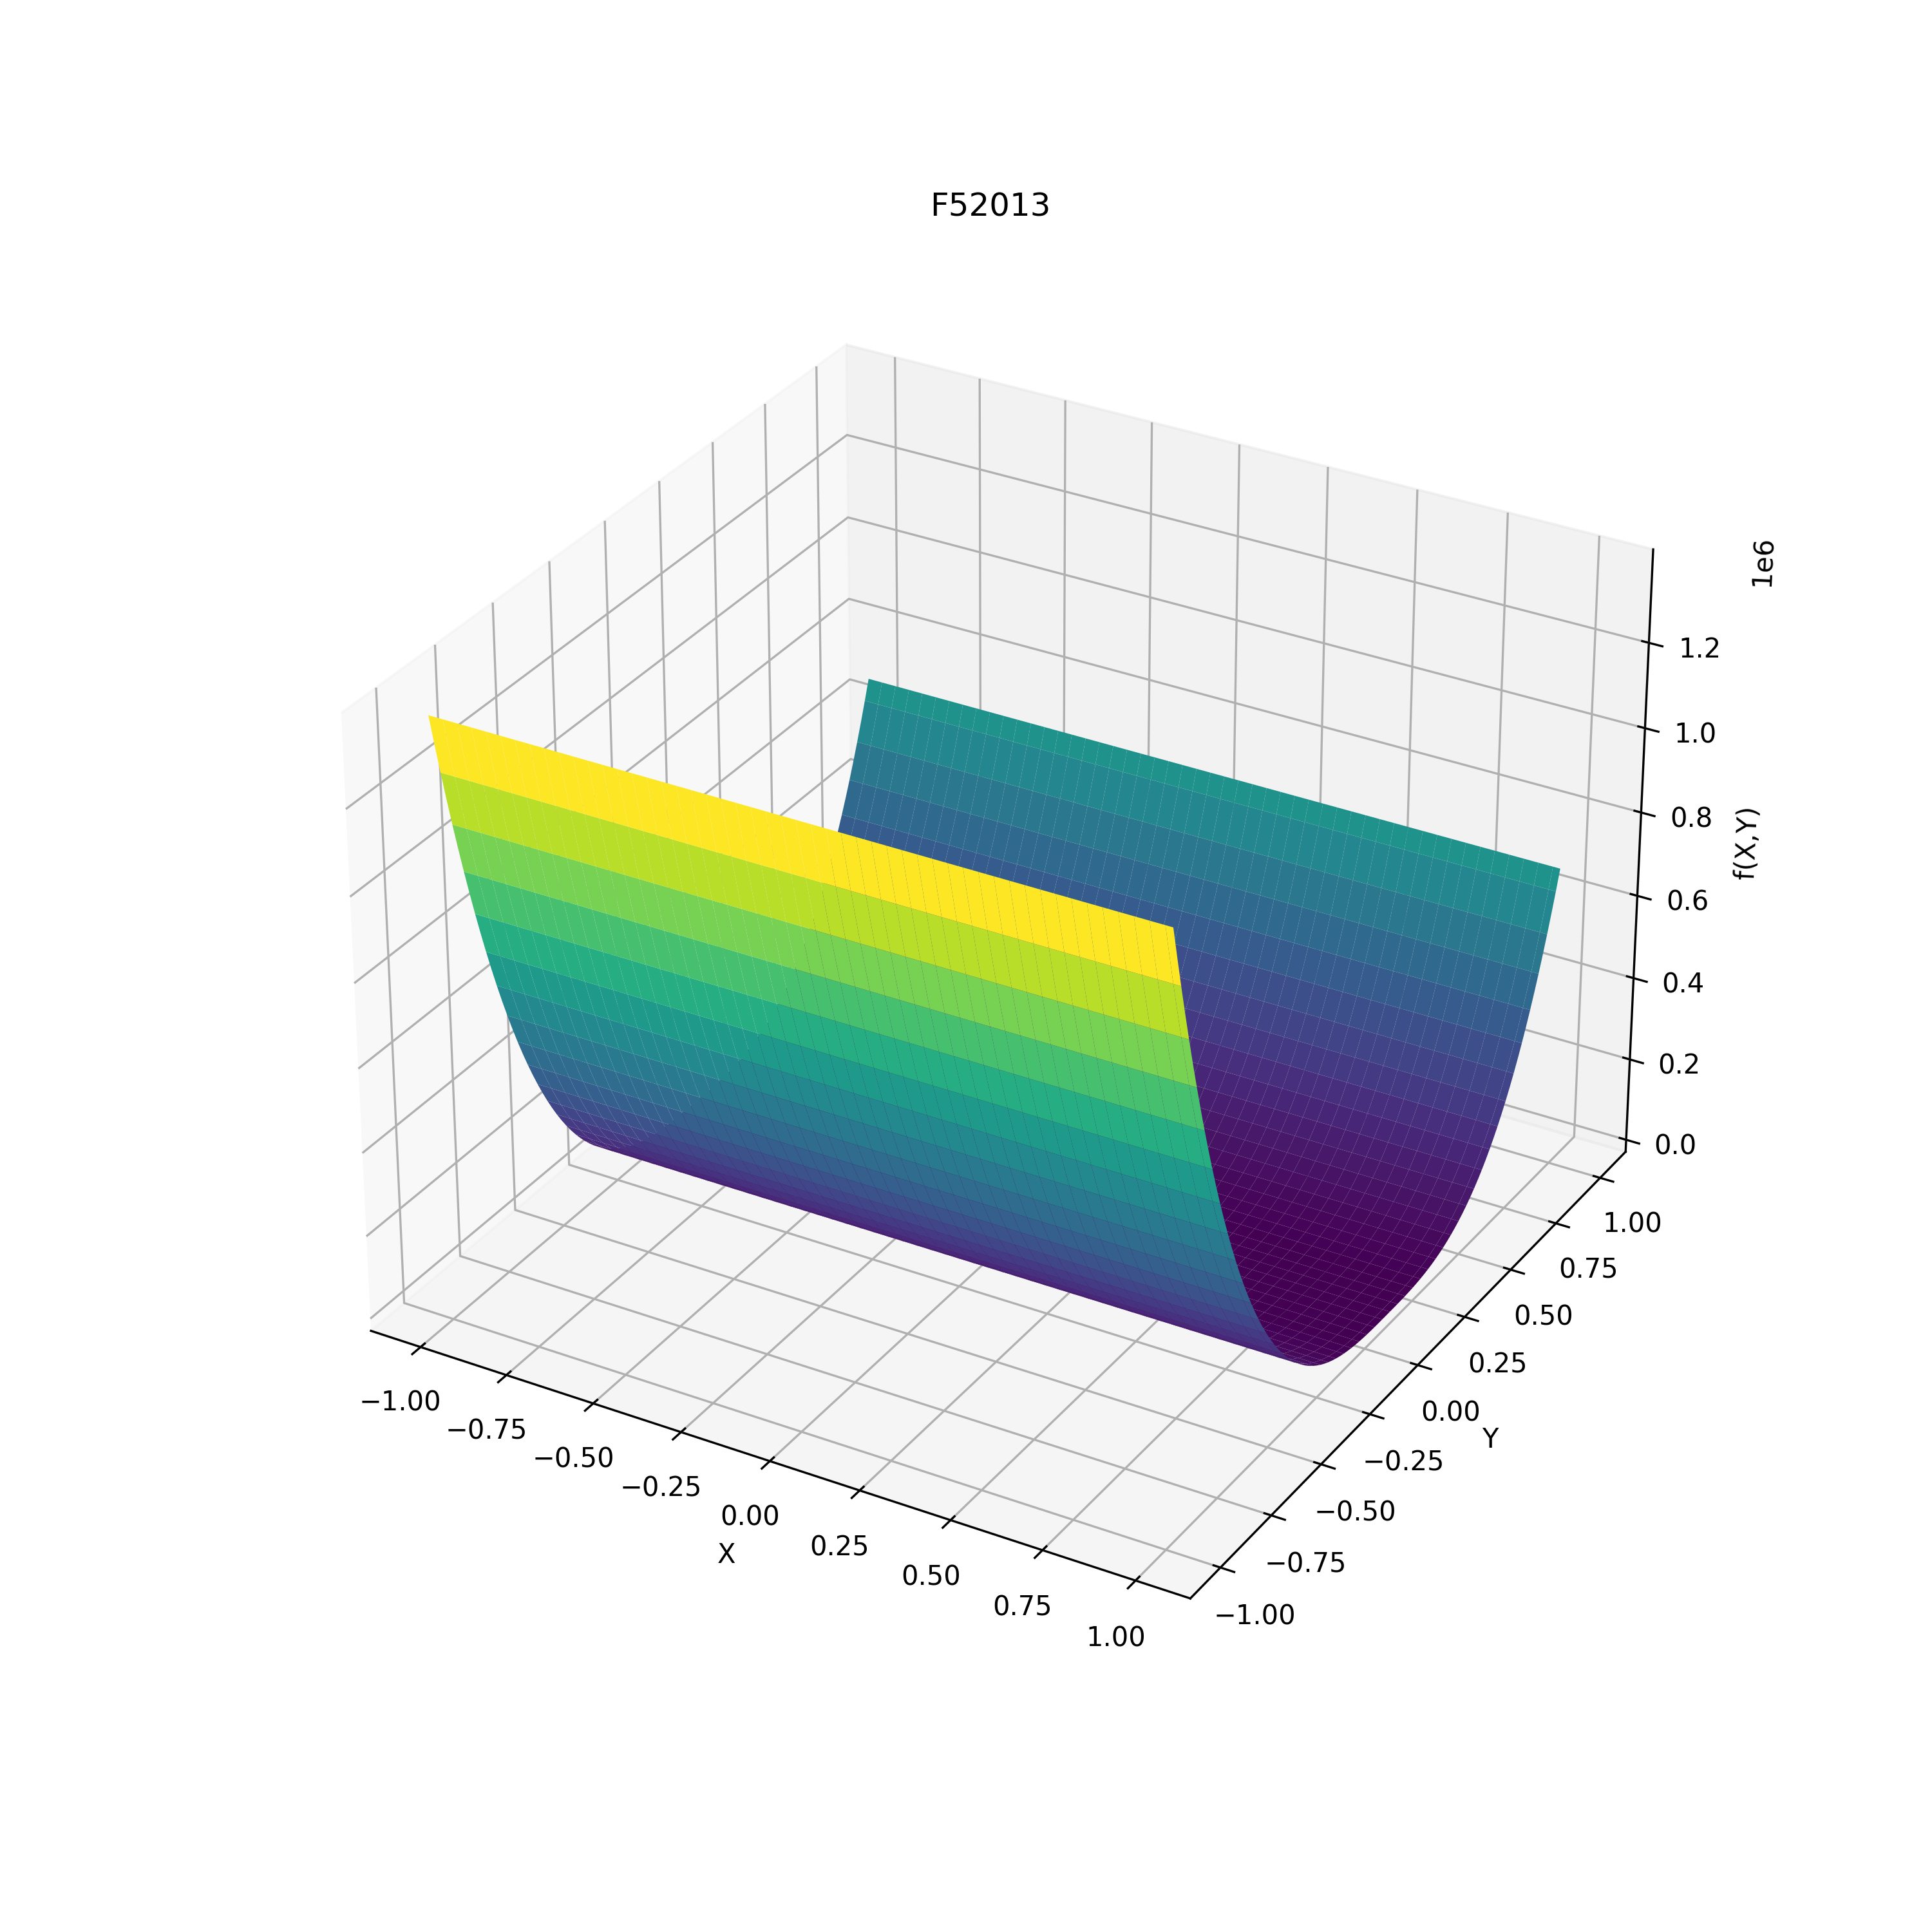
\includegraphics[height=3cm, keepaspectratio]{met_an/cec/funkcje/F52013.png}
%     \end{subfigure}
%     \hfill
%     \begin{subfigure}[c]{0.7\textwidth}
%         \centering
%         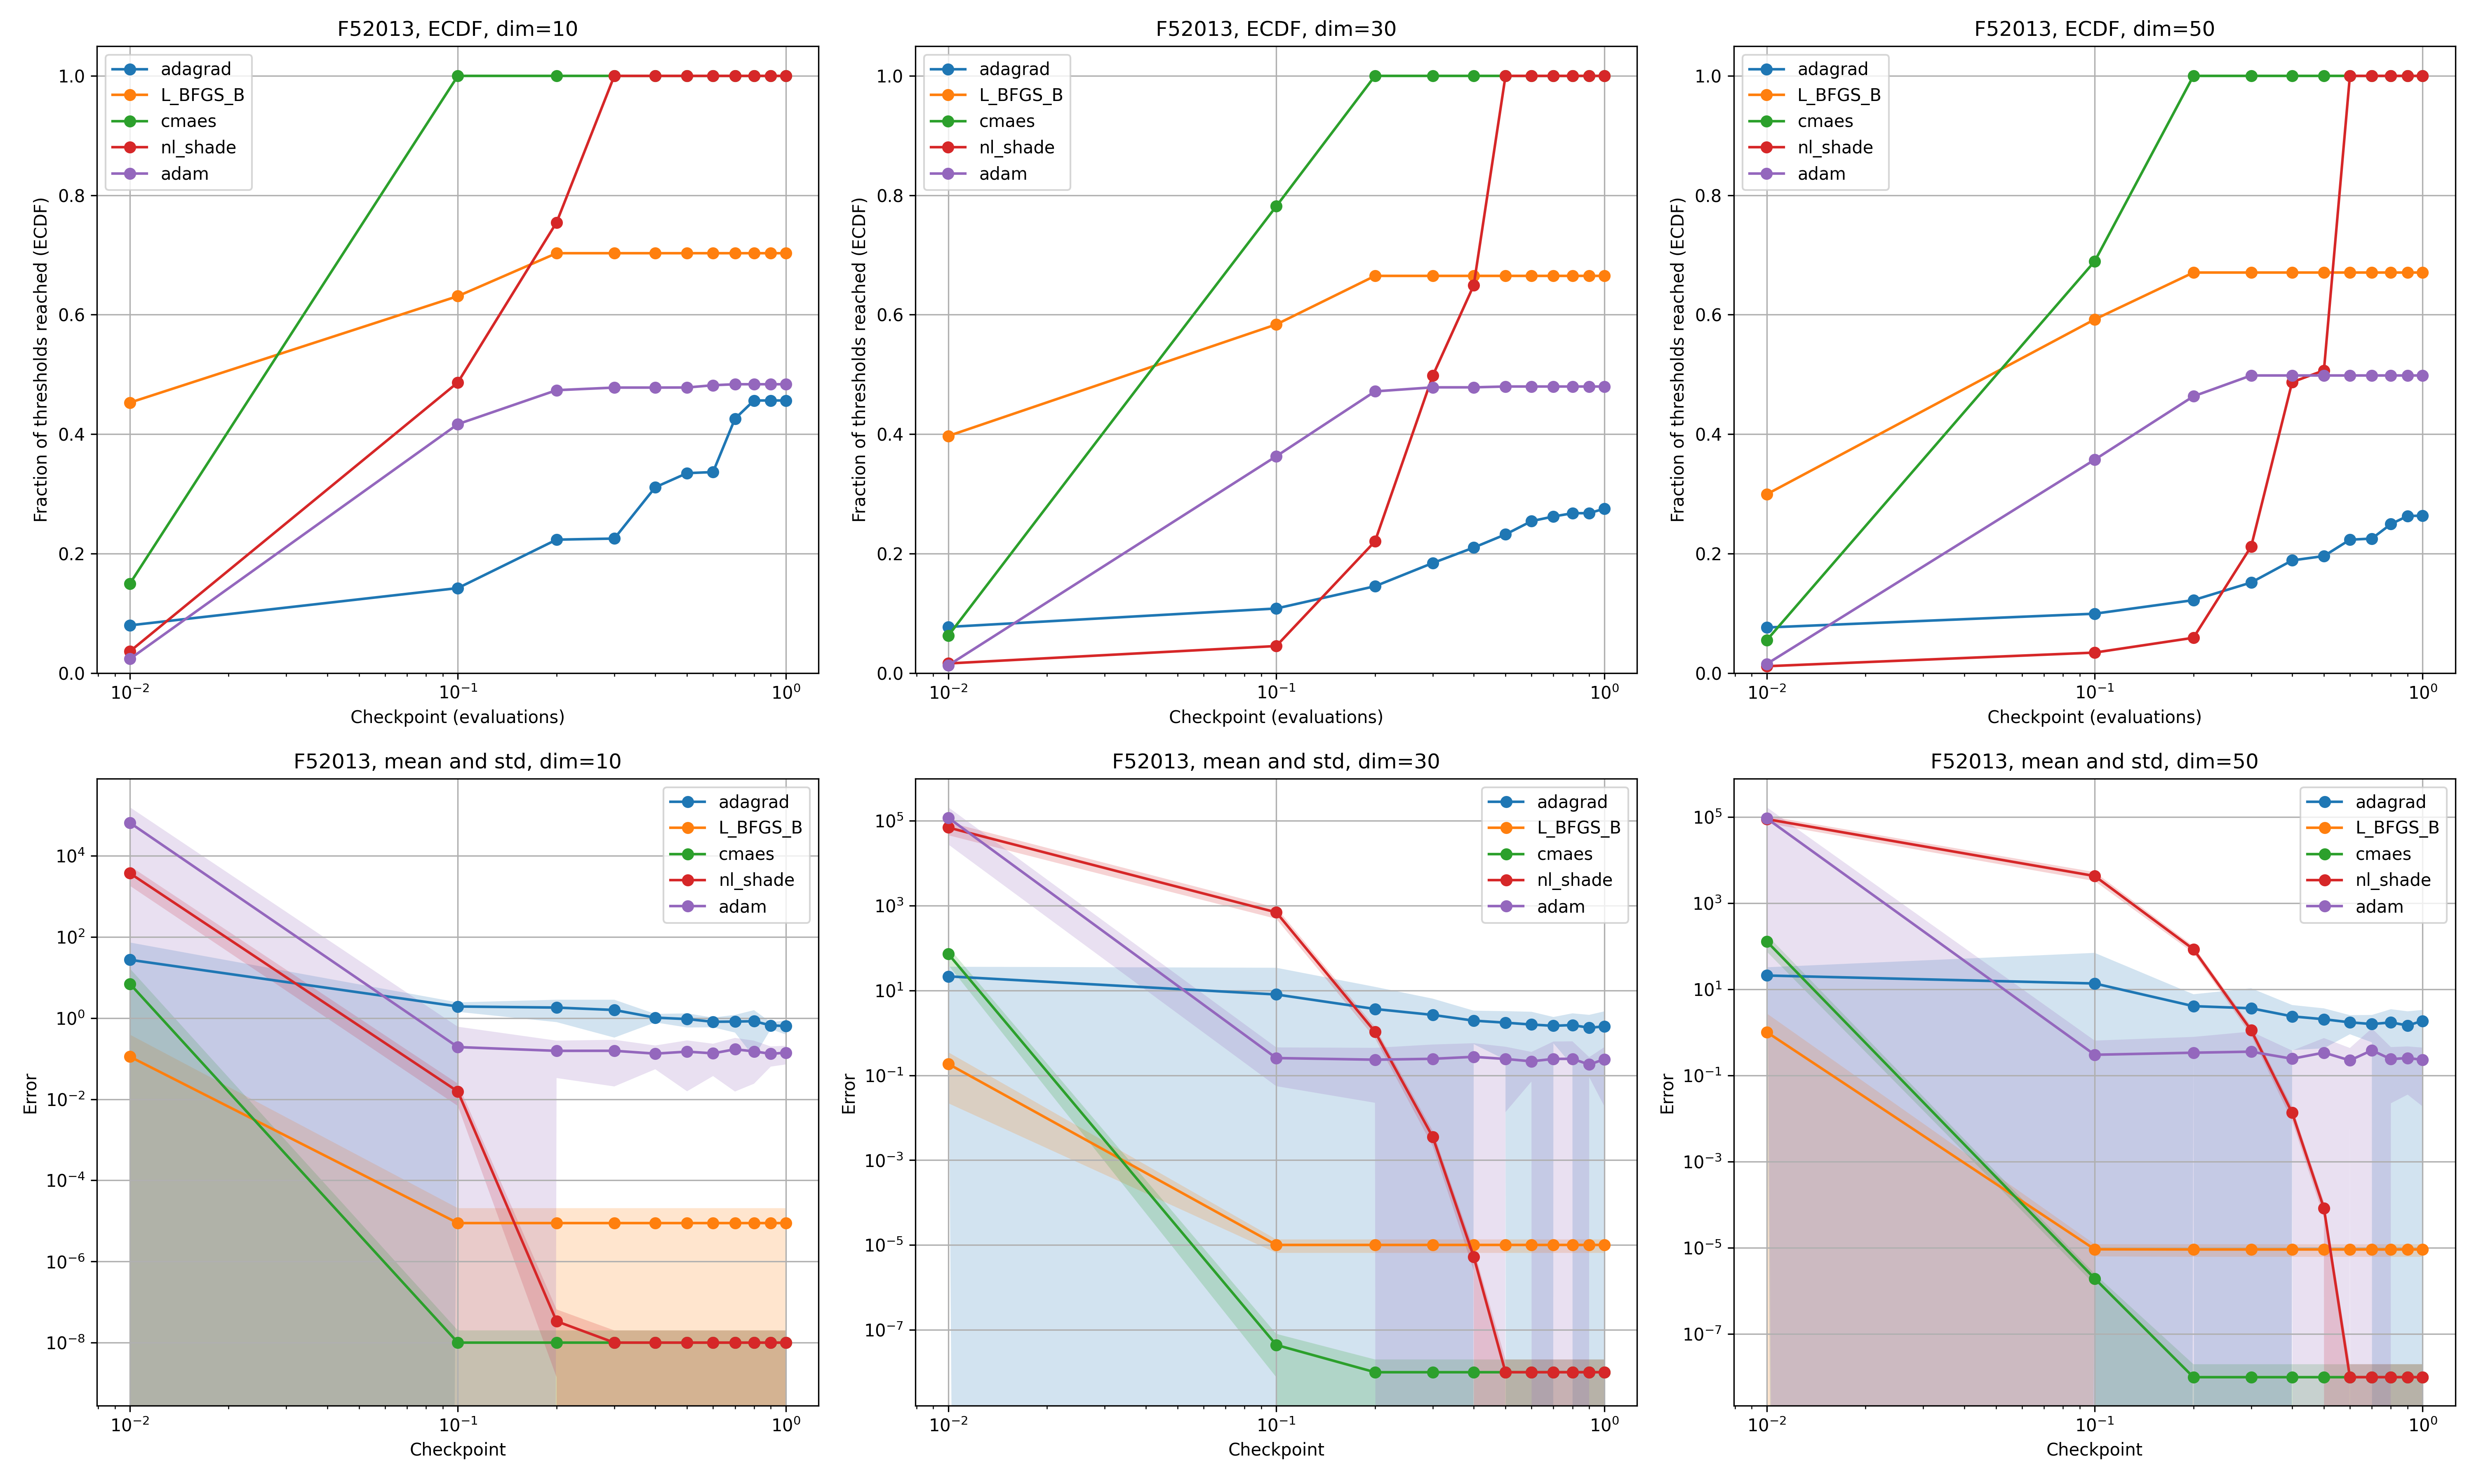
\includegraphics[height=6.5cm, keepaspectratio]{met_an/cec/funkcje/F52013_rec.png}
%     \end{subfigure}
%     \caption{Different Powers Function}
%     \label{fig:F52013}
% \end{figure}

% \begin{figure}[H]
%     \centering
%     \begin{subfigure}[c]{0.2\textwidth}
%         \centering
%         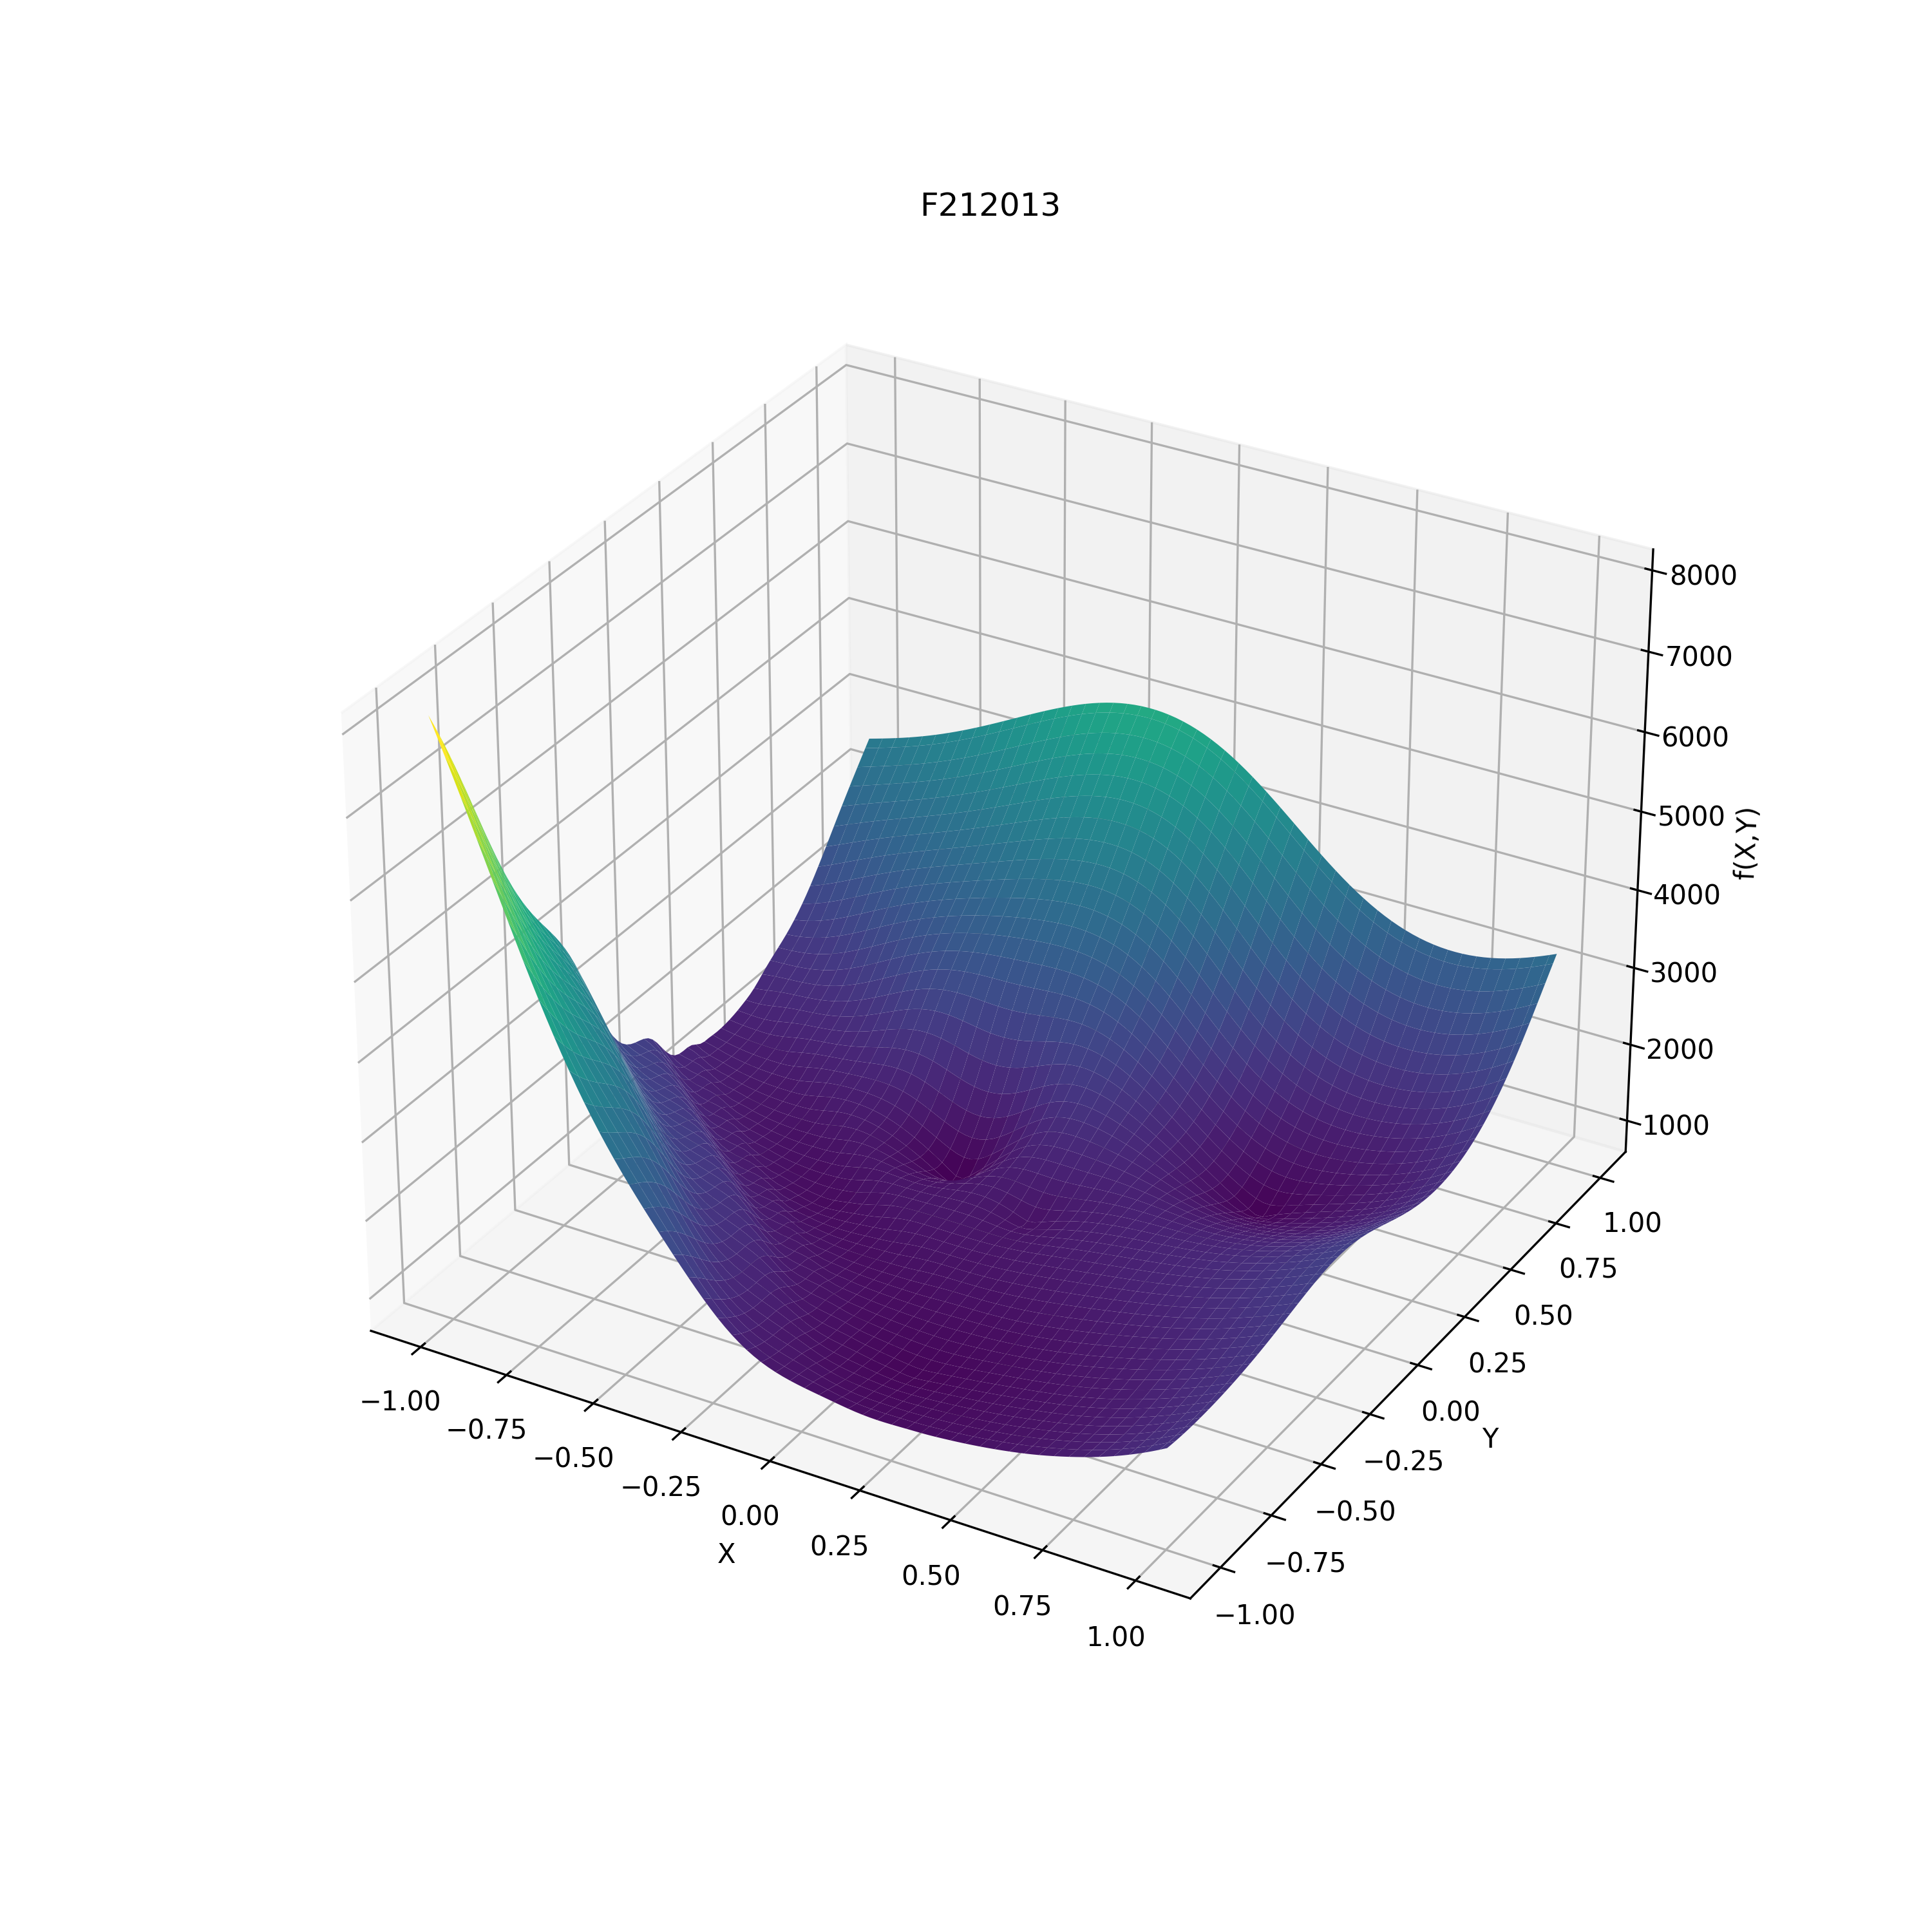
\includegraphics[height=3cm, keepaspectratio]{met_an/cec/funkcje/F212013.png}
%     \end{subfigure}
%     \hfill
%     \begin{subfigure}[c]{0.7\textwidth}
%         \centering
%         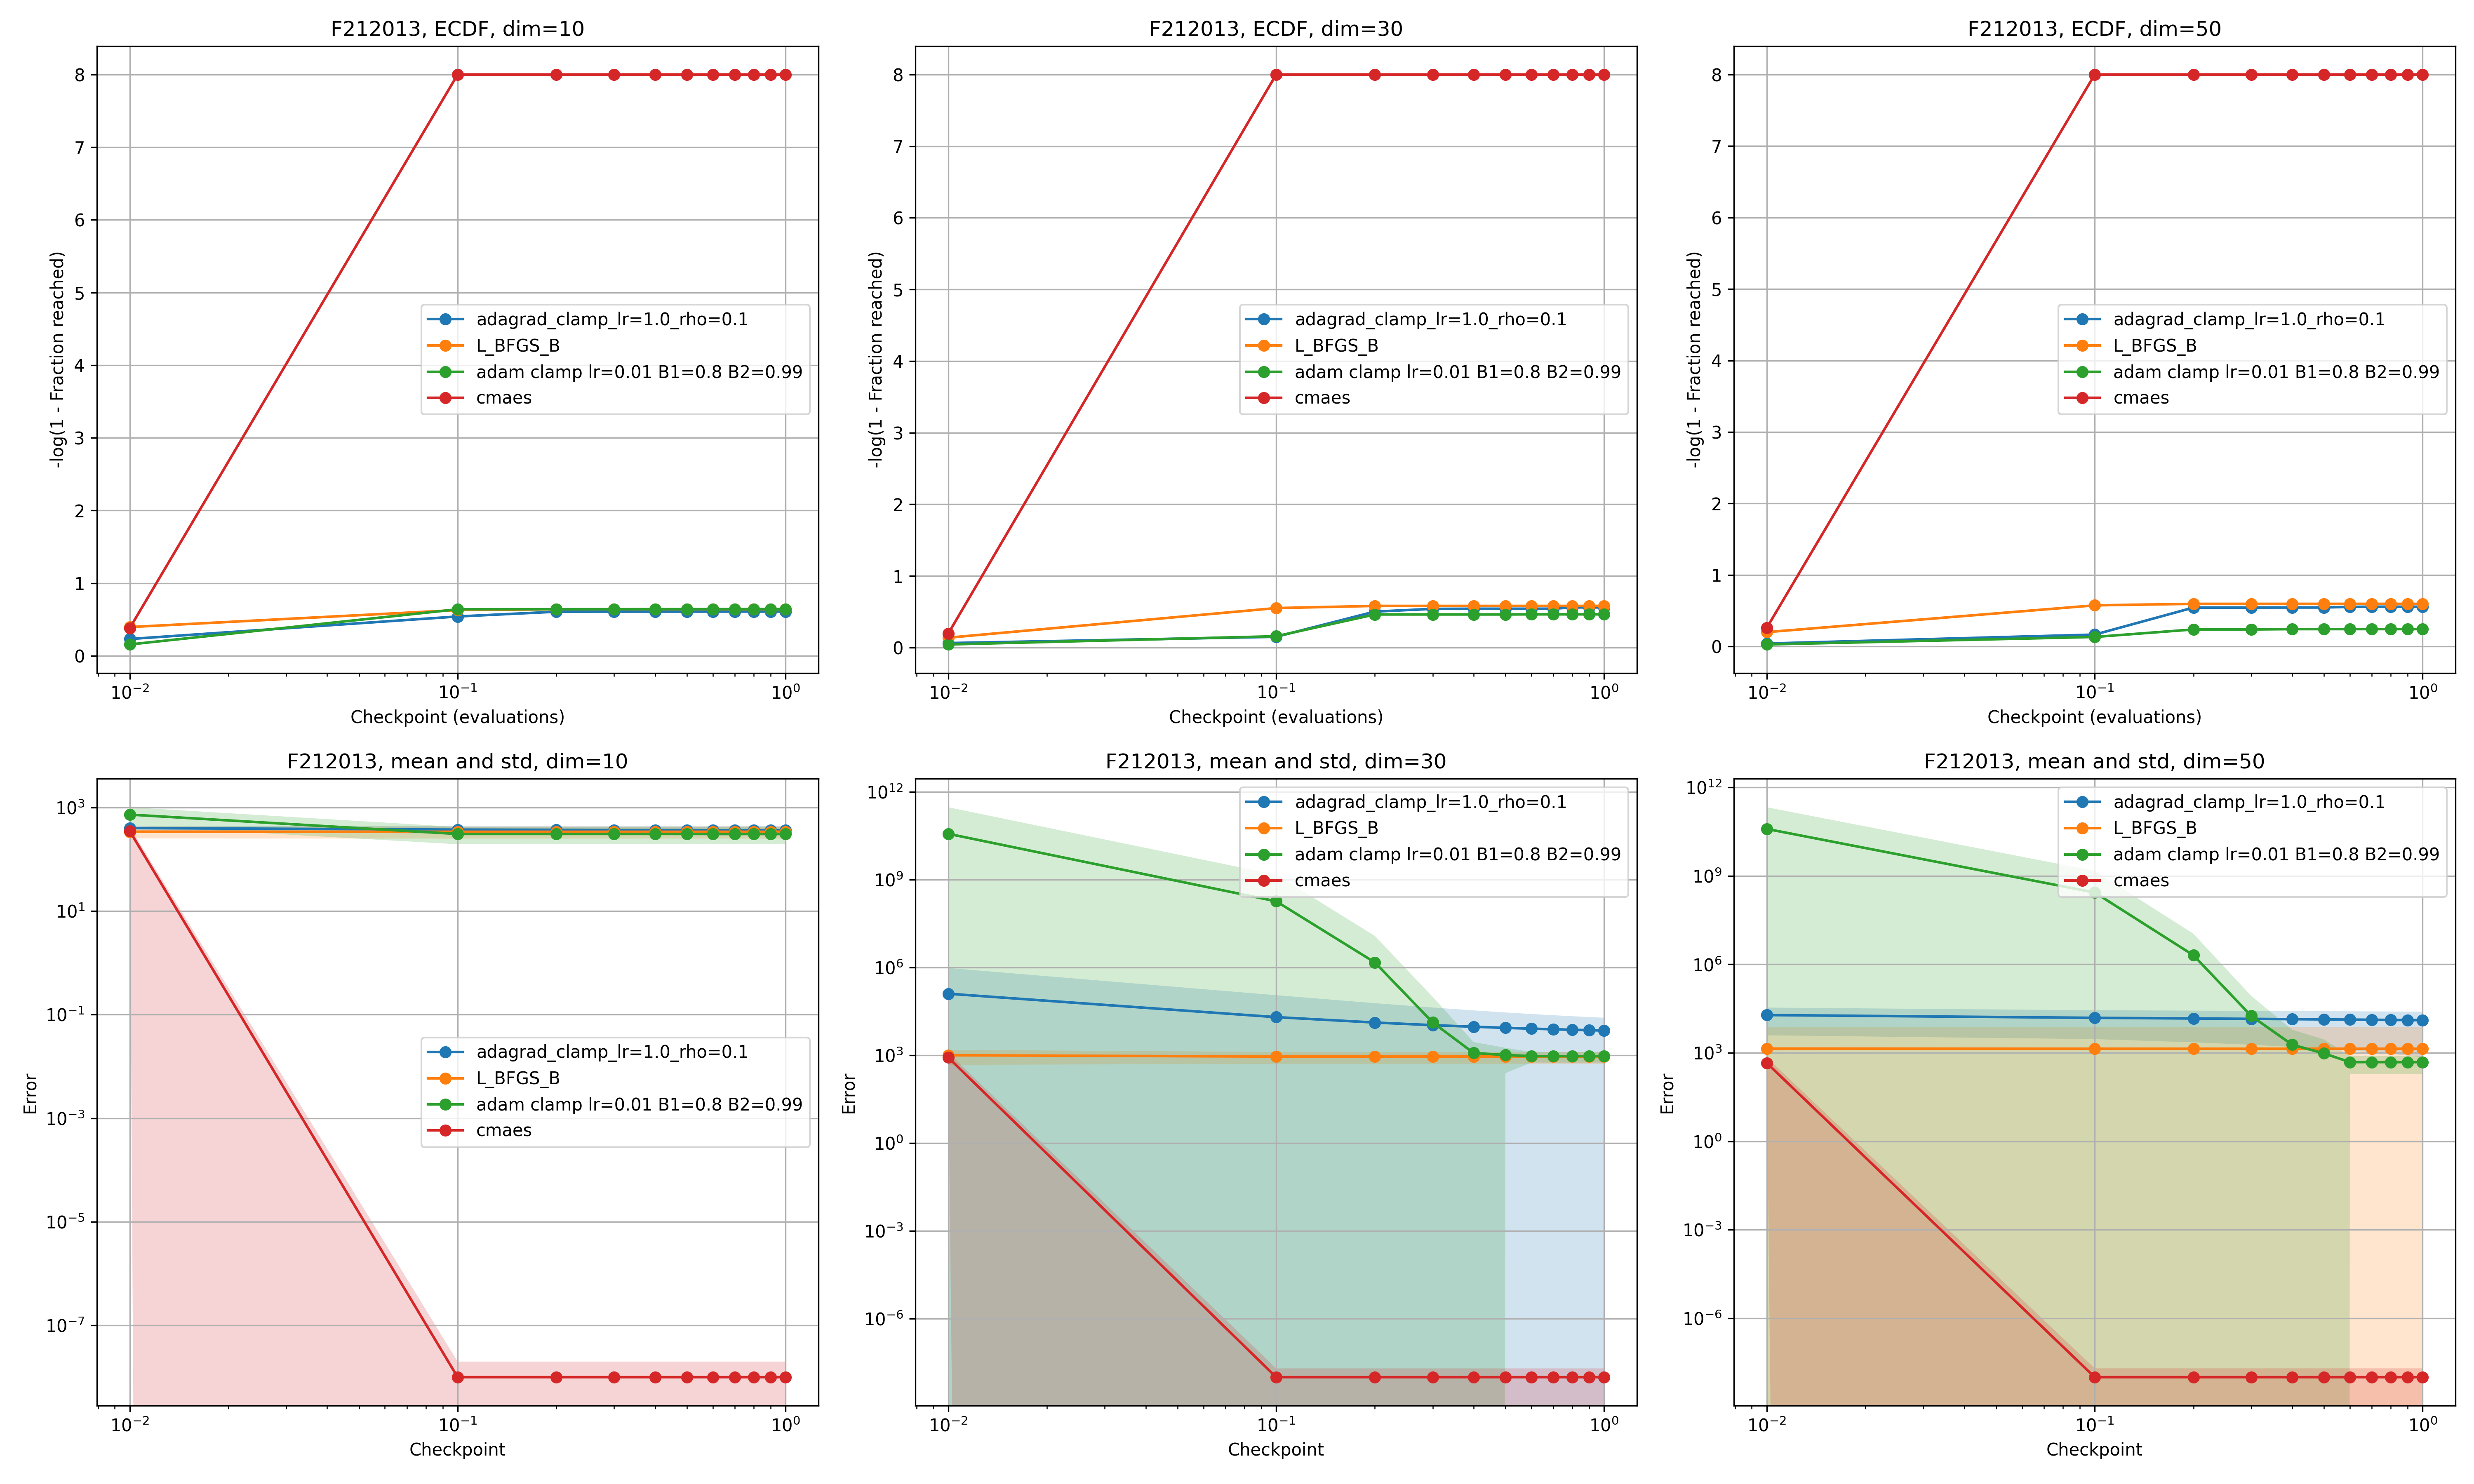
\includegraphics[height=6.5cm, keepaspectratio]{met_an/cec/funkcje/F212013_rec.png}
%     \end{subfigure}
%     \caption{Composition Function 1 (n=5,Rotated)}
%     \label{fig:F212013}
% \end{figure}



% \begin{figure}[H]
%     \centering
%     \begin{subfigure}[c]{0.2\textwidth}
%         \centering
%         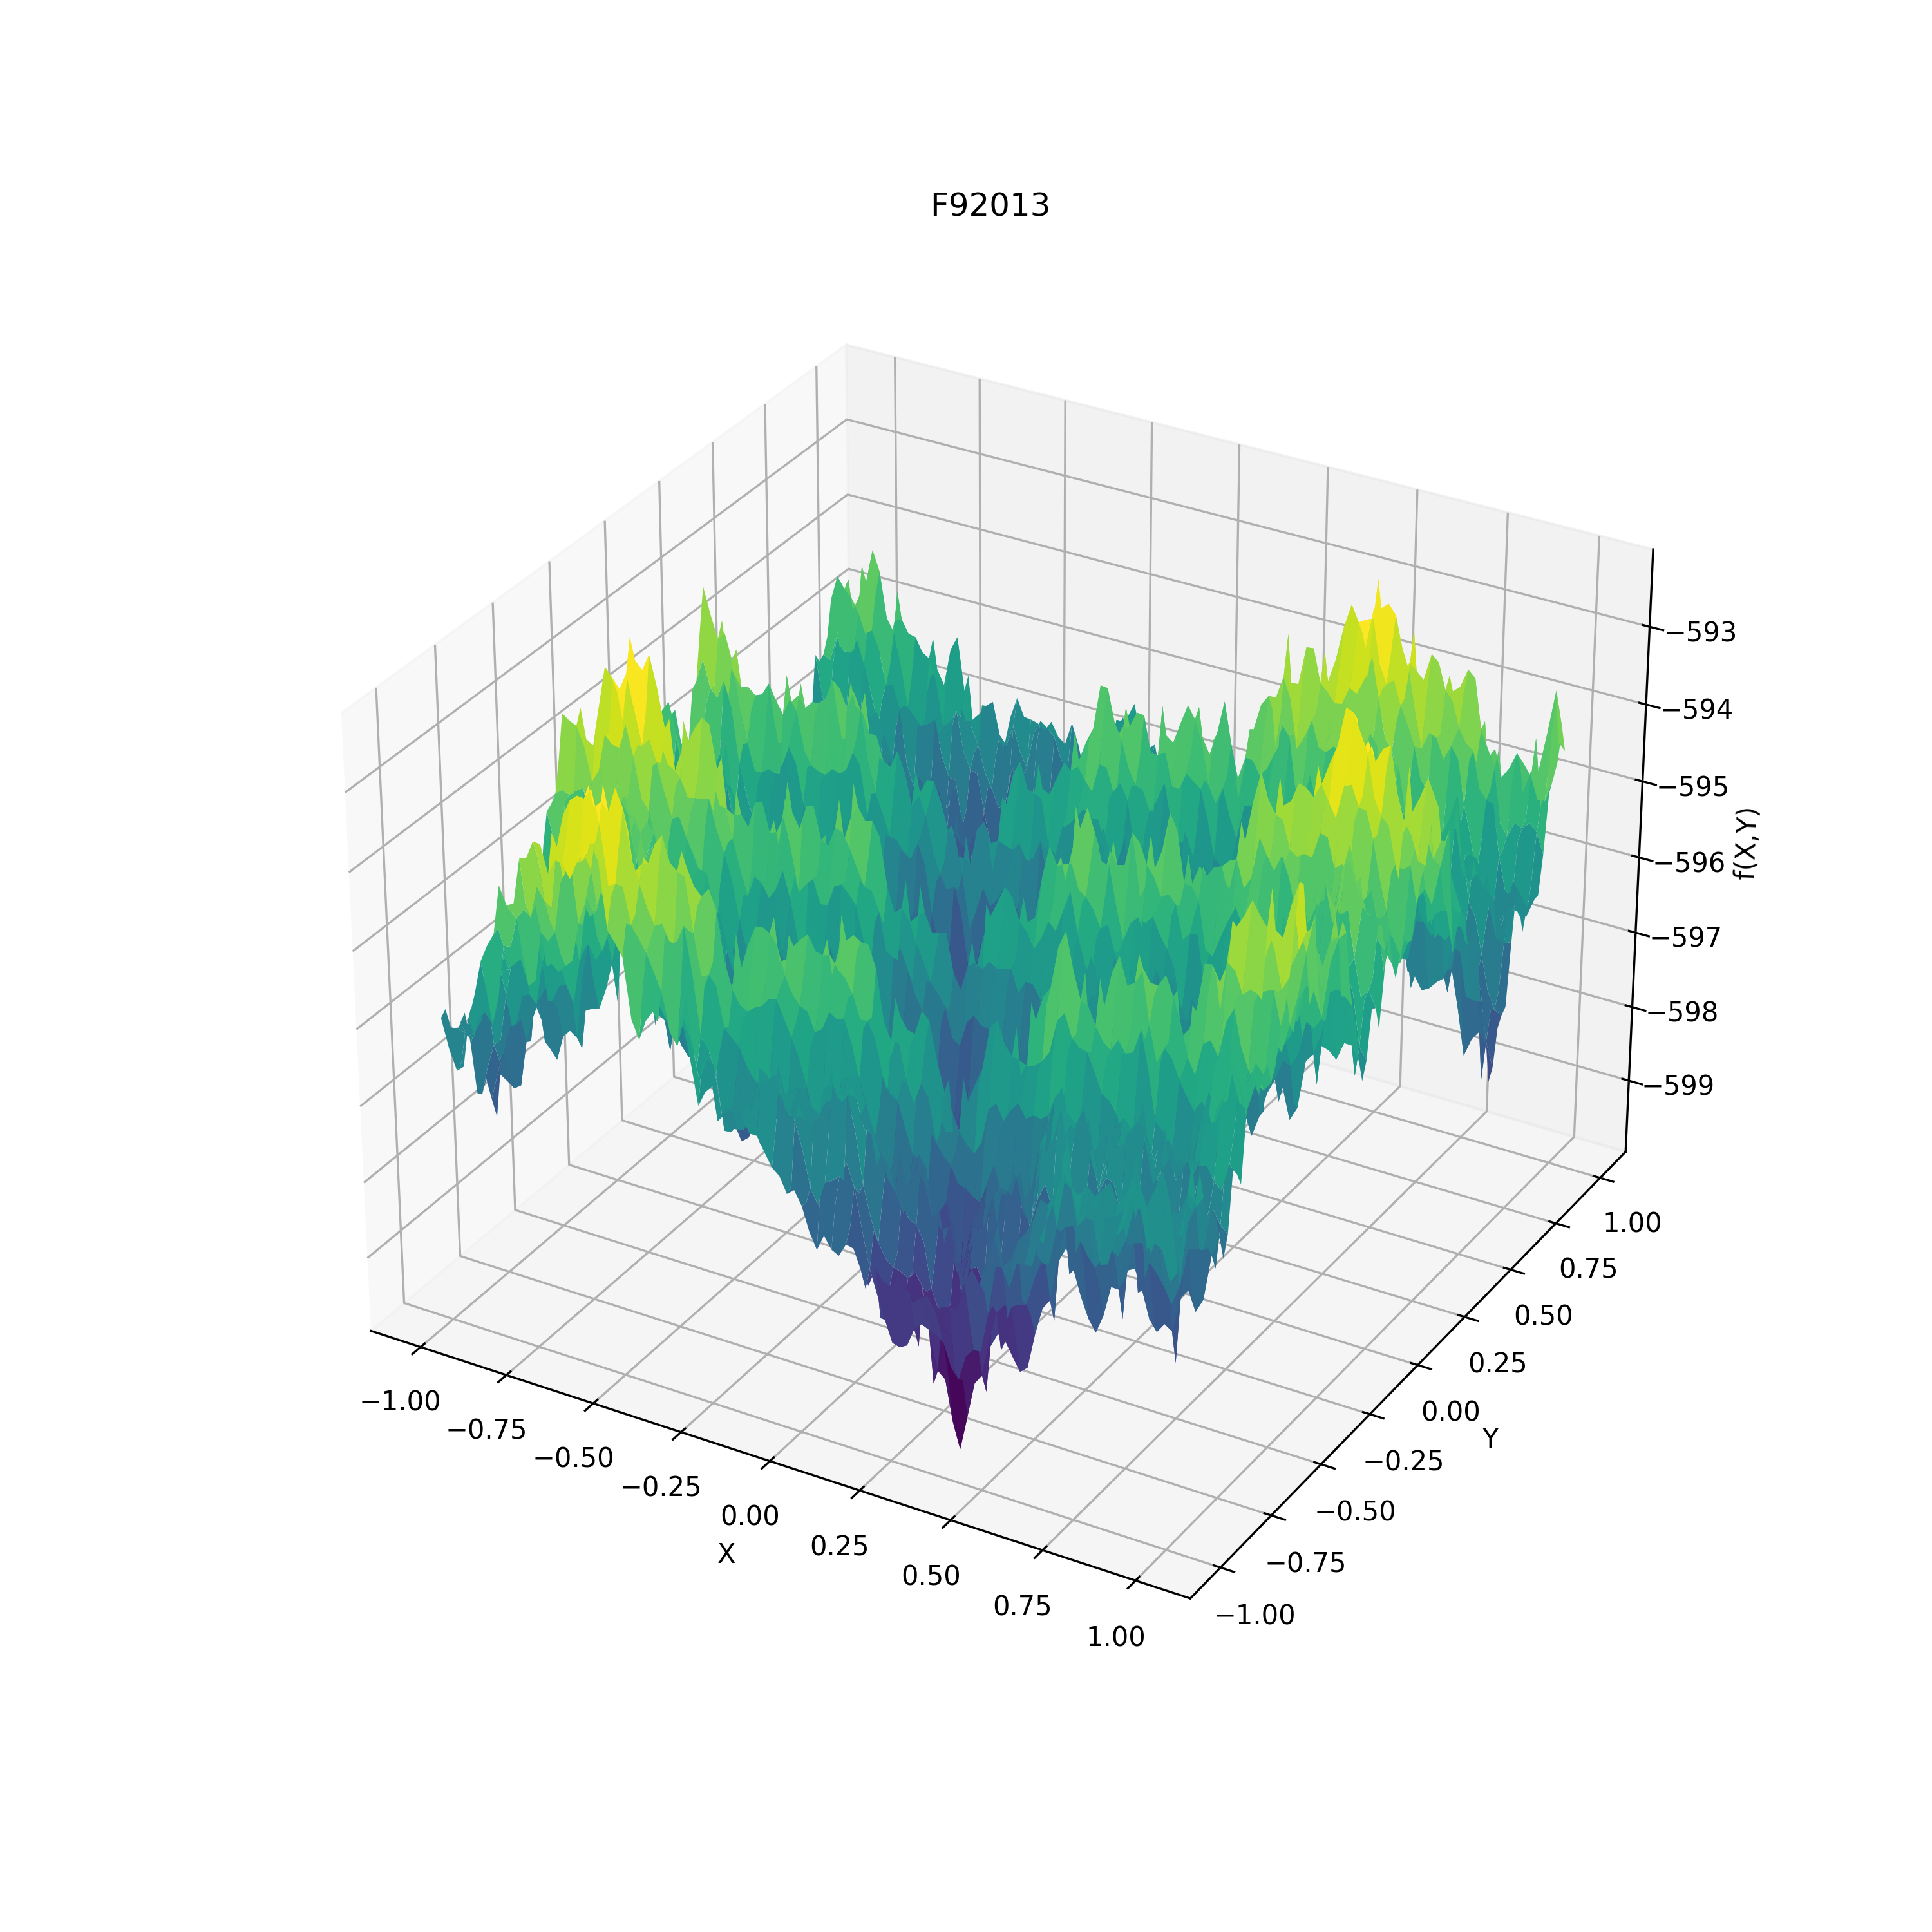
\includegraphics[height=3cm, keepaspectratio]{met_an/cec/funkcje/F92013.png}
%     \end{subfigure}
%     \hfill
%     \begin{subfigure}[c]{0.7\textwidth}
%         \centering
%         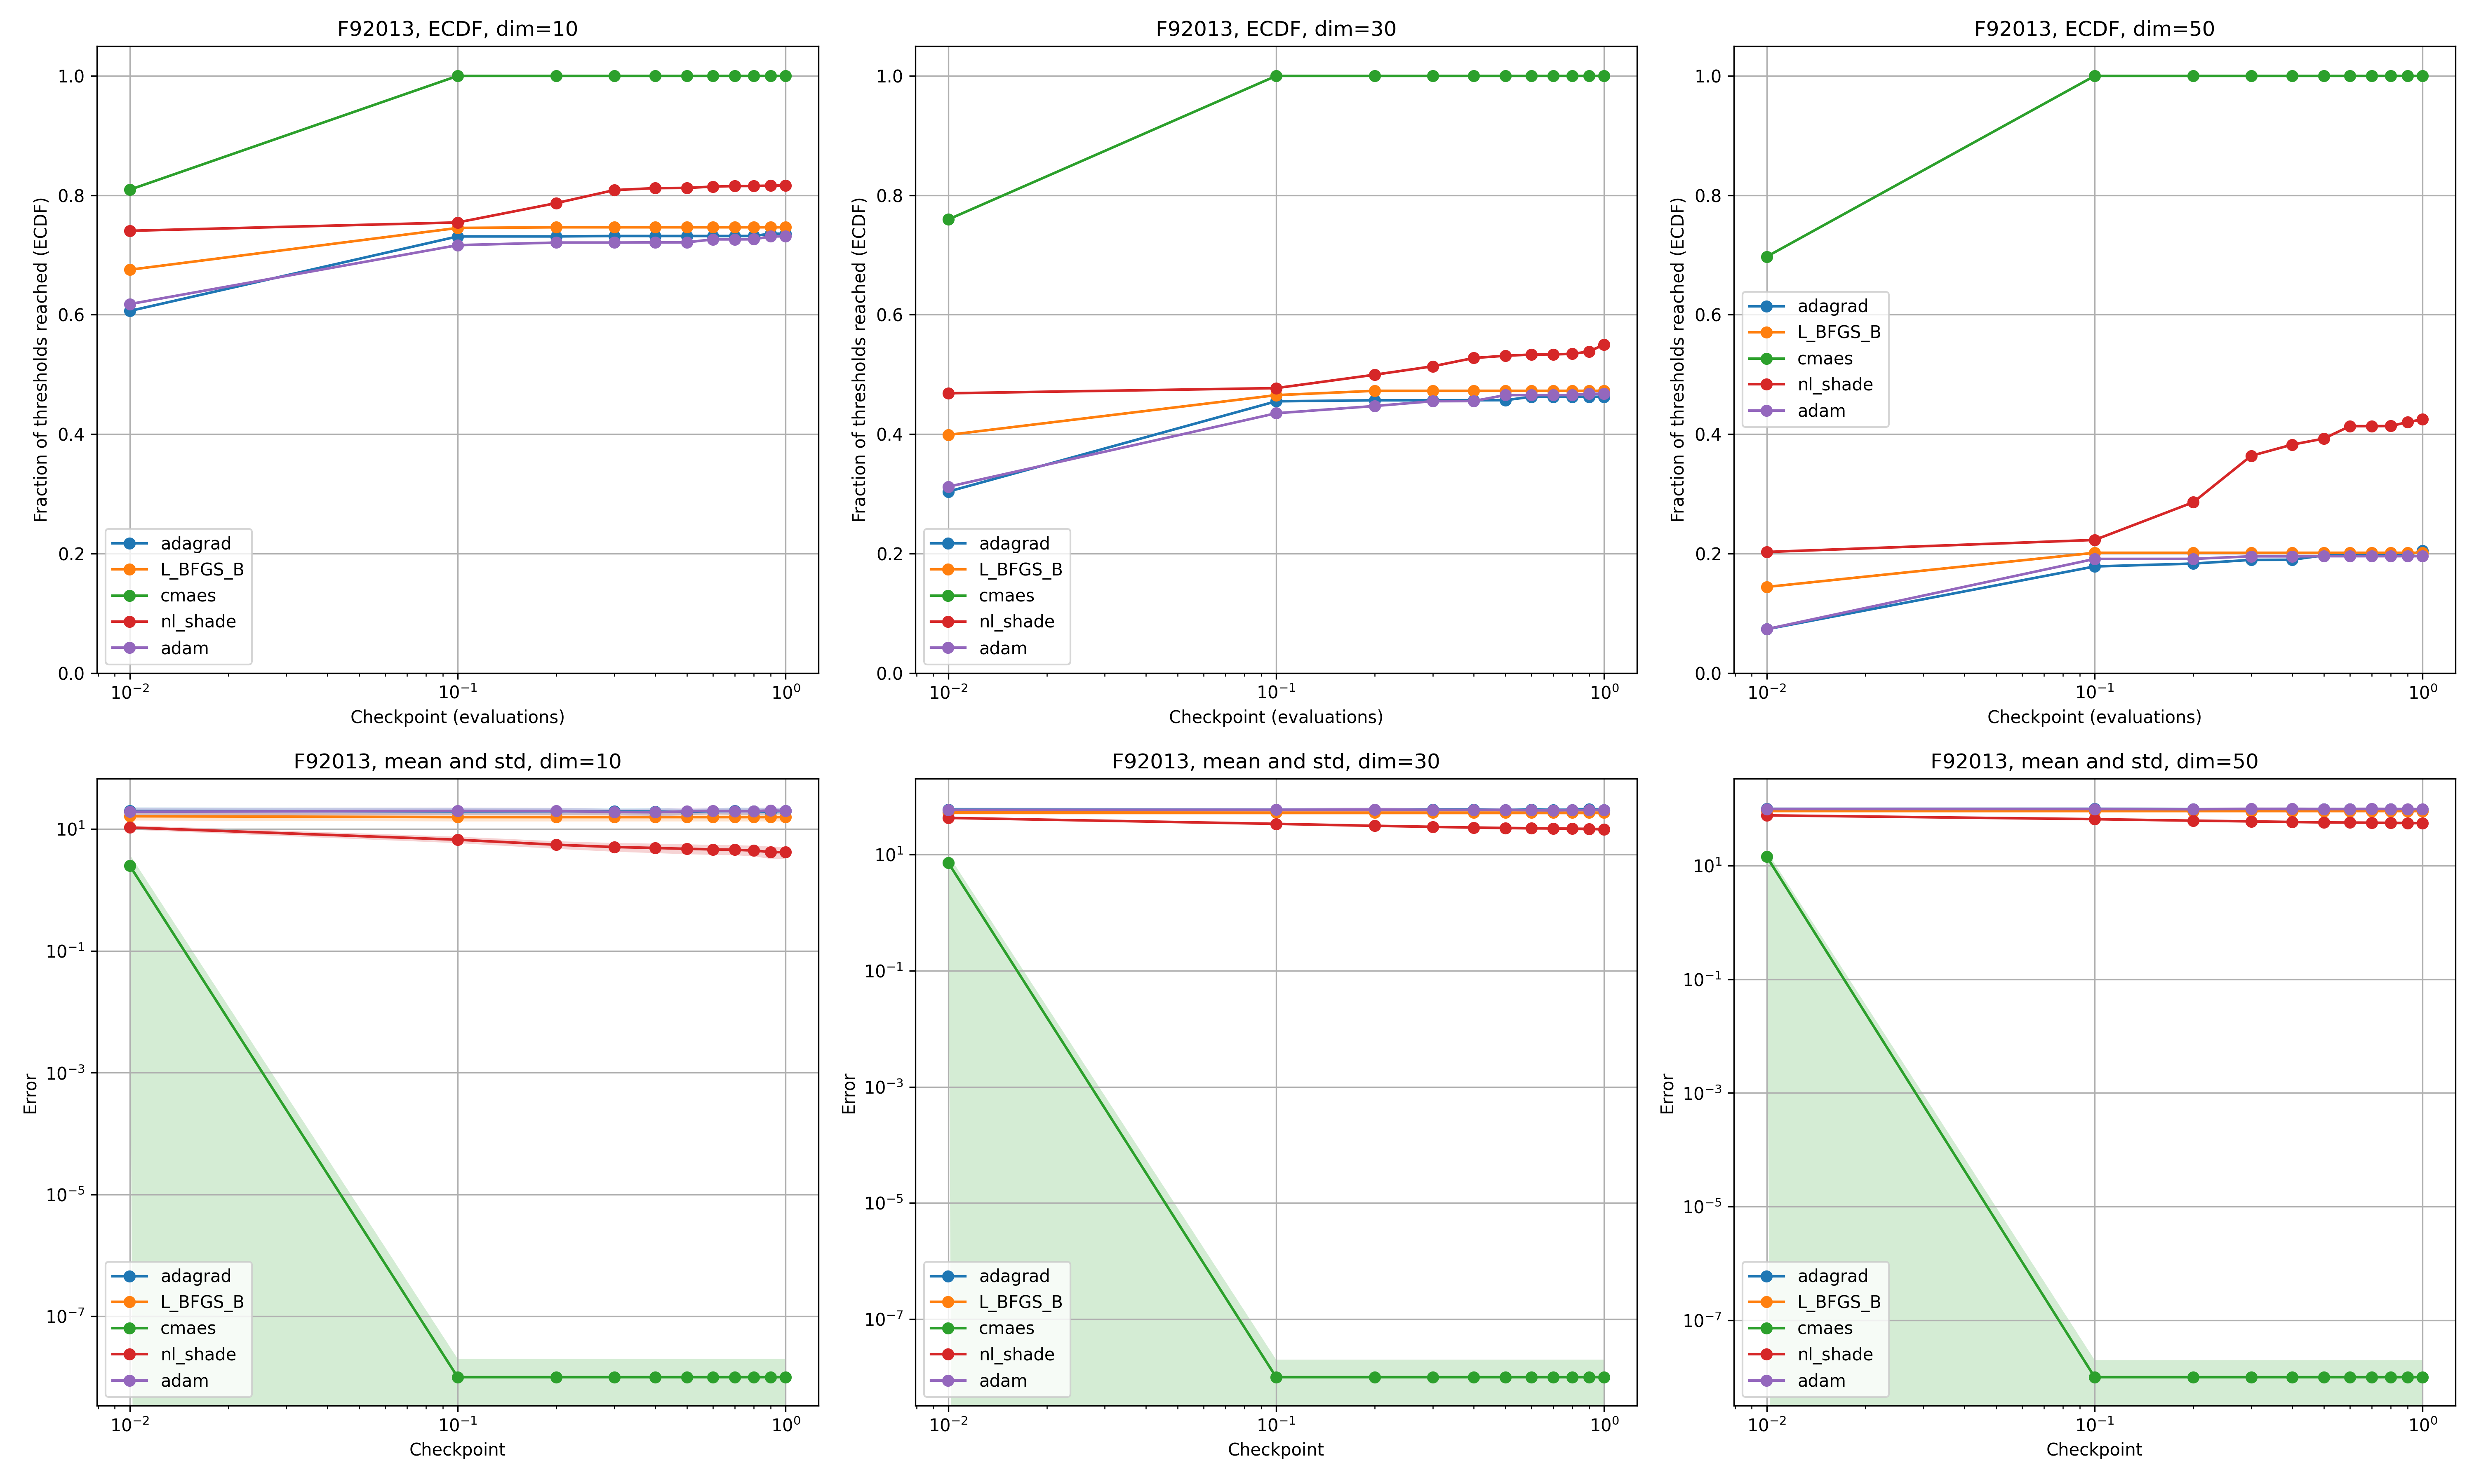
\includegraphics[height=6.5cm, keepaspectratio]{met_an/cec/funkcje/F92013_rec.png}
%     \end{subfigure}
%     \caption{Rotated Weierstrass Function}
%     \label{fig:F92013}
% \end{figure}

